% Chapter generated from c0bd7425-paper1.tex
% chapter macros
\DeclareRobustCommand{\PD}{\mathrm{PD}}
\DeclareRobustCommand{\GEM}{\mathrm{GEM}}
\DeclareRobustCommand{\Be}{\mathrm{Be}}
\DeclareRobustCommand{\E}{\mathbb{E}}
\DeclareRobustCommand{\Prob}{\mathbb{P}}
\DeclareRobustCommand{\Var}{\mathrm{Var}}
\DeclareRobustCommand{\Cov}{\mathrm{Cov}}
\DeclareRobustCommand{\R}{\mathbb{R}}
\DeclareRobustCommand{\dd}{\,\mathrm{d}}
\chapter{Many Parameter Models in Population Genetics}\label{ch:mp}
\chaptermark{Many Parameter Models}
\begin{chaptersummary}
Population genetics has become a many parameter subject. Whole genome average effects,
polygenic effect sizes and allelic frequency spectra all involve parameter counts that are
large relative to any sample, and in Fisher's whole genome formulation the count is
astronomically large. We make three points. First, Fisher's definition of the average
effect, as restated by \citet{mp:ewens2024}, is a weighted least squares projection, and the
plug in additive genetic variance obtained from a linear smoother $H$ carries a noise term
$\sigma^2\,\mathrm{tr}(H^\top H)/N$, which for the unregularised fit of that projection is an inflation of exactly
$p\sigma^2/N$. Second, the natural prior for such problems is a species sampling prior in
the sense of \citet{mp:kingman1975}, of which the Ewens Sampling Formula is the canonical member.
Third, the global local shrinkage priors of sparse Bayesian statistics and the
two parameter Poisson Dirichlet family are linked by an exact identity of marginal laws: if $\kappa\sim\Be(a,b)$ is the
shrinkage weight of a prior in the three parameter beta normal class, then $\kappa$ has the law of the
first stick breaking weight of $\GEM(1-a,\,a+b-1)$, and the mean intensity of the matched frequency spectrum is
$\nu(x)=x^{-1}f_\kappa(x)$ exactly; the full partition laws are not shown to agree. Sparsity level is Pitman's $\alpha$. We then prove the resulting rate directly for the
shrinkage prior as used: at the canonical global scale $\tau_n=n^{-1/2}$ the expected
effective model size is $\asymp n^{1-a}$, matching the Poisson Dirichlet discovery rate in
exponent exactly and in constant to within $\Gamma(2-a)\in[0.8856,1]$. The horseshoe and the
Strawderman Berger prior therefore sit at $n^{1/2}$, while the uniform shrinkage prior and
the other priors with $a=1$ sit at $\log n$ (Laplace type priors, outside the beta normal class, stay bounded), and the conventional choice of global
scale is the unique power of $n$ at which the two sides agree for every $a$. We give proofs, worked one locus and two locus examples, a
small design on which the optimism can be checked by hand, a worked Kingman
correspondence at $n=3$, a table of discovery counts for three members of the beta normal
class, a conjugate augmentation for the mutation parameter with worked small sample and
butterfly examples, and simulations. In an epistatic
whole genome simulation with $L=400$ loci the unregularised projection in its orthogonal design form inflates
$\sigma_A^2$ by a factor of $3.09$ at $N=200$; a species sampling prior at the global scale the
theory identifies, with no oracle input, never inflates it and reaches $0.98$ of the truth by
$N=3200$.
\end{chaptersummary}
\section{Introduction}

\citet{mp:ewens2024} opens with the observation that the direction of research in population
genetics theory is now, and correctly, retrospective, and that this is driven by the volume
of genomic data available. That change of direction has a statistical consequence which has
not been much discussed. Retrospective inference from genomic data is inference in models
whose parameter count is large relative to the sample, often very large, and sometimes
astronomically large. The classical prospective theory was developed for models with a
handful of parameters and its estimators inherit no protection against the difficulties that
arise when parameter count grows with, or exceeds, the amount of data.

This chapter is about what to do in that regime, and about the fact that population genetics
already contains, in the Ewens Sampling Formula, the prior distribution that the statistics
literature spent the last twenty years rediscovering under a different name.

We organise the argument around three questions.

\begin{enumerate}[leftmargin=1.6em]
\item \emph{Is the additive genetic variance safe to estimate by plugging in?} No.
Fisher's definition of the average effect, restated by \citet[Equation 10]{mp:ewens2024}, is a
weighted least squares projection onto an additive subspace whose dimension is of the order of the number of
alleles in the genome. Section \ref{mp:sec:avgeff} shows that fitting that projection produces
an estimate of $\sigma_A^2$ exceeding the truth in expectation by $p\sigma^2/N$, where $p$
is the number of fitted average effects. This is the optimism that inflates $R^2$ in any
regression, and at genomic parameter counts it is not a small correction.
\item \emph{What is the right prior?} Section \ref{mp:sec:kingman} argues that the right
prior is a species sampling prior. \citet{mp:kingman1975} introduced the random discrete
distributions obtained by normalising a subordinator and showed that sampling from one induces an
exchangeable partition. The Ewens Sampling Formula is the partition induced by the gamma
subordinator, and the global local shrinkage priors of \citet{mp:carvalho2010} and
\citet{mp:polson2012} are built from subordinator increments, without the normalisation.
\item \emph{How far does the correspondence go?} Section \ref{mp:sec:main} gives our main
results. Theorem \ref{mp:thm:main} identifies the shrinkage weight of the three parameter beta
normal family with the first stick breaking weight of a two parameter Poisson Dirichlet
process. Theorem \ref{mp:thm:spectrum} shows the identification is not confined to one weight:
the entire frequency spectrum intensity is the shrinkage density with its size bias removed. Corollary
\ref{mp:cor:growth} converts this into discovery rates.
\end{enumerate}

Section \ref{mp:sec:wls} explains how the resulting estimators relate to Fisher's own weighted
least squares criterion, Section \ref{mp:sec:conj} treats inference for the mutation parameter,
Section \ref{mp:sec:num} reports simulations, Section \ref{mp:sec:genetics} draws out the genetic
consequences and Section \ref{mp:sec:disc} concludes. Proofs not given in the text are
collected in Section \ref{mp:app:proofs}, and Section \ref{mp:sec:ex} contains exercises.

\subsection{Methodological contribution}
\label{mp:sec:contrib}

The chapter draws on two literatures which do not usually meet, so we state at the outset what
is on offer.

\begin{enumerate}[leftmargin=1.8em,itemsep=3pt]
\item \emph{An identification, Theorem \ref{mp:thm:main}.} The shrinkage weight of a
global local prior in the three parameter beta normal class is the first stick breaking
weight of a two parameter Poisson Dirichlet process, under the explicit bijection
$(\alpha,\theta)=(1-a,\,a+b-1)$. The horseshoe is $\PD(1/2,0)$, the Strawderman Berger
prior is $\PD(1/2,1/2)$, and the uniform shrinkage prior is the Ewens Sampling Formula at
$\theta=1$.
\item \emph{An extension of that identification to the whole spectrum, Theorem
\ref{mp:thm:spectrum}.} The mean intensity of allele frequencies is $\nu(x)=x^{-1}f_\kappa(x)$,
the shrinkage density with its size bias removed, from which Fisher's log series follows as the case
$\kappa\sim\Be(1,\theta)$.
\item \emph{A design rule, Corollary \ref{mp:cor:growth}, proved directly for the shrinkage
prior in Theorem \ref{mp:thm:effsize}.} The number of variants a prior will ever declare grows
like $n^{1-a}$, and the effective model size of \eqref{mp:eq:gl} at the canonical global scale
$\tau_n=n^{-1/2}$ has the same exponent with a constant agreeing to within
$\Gamma(2-a)\in[0.8856,1]$. Choosing a prior is therefore choosing a discovery rate,
and the choice is a genetic statement about the polygenic architecture, not a computational
convenience.
\item \emph{A bias calculation for Fisher's own estimand, Proposition
\ref{mp:prop:optimismgen} and Corollary \ref{mp:prop:optimism}.} The plug in additive genetic
variance obtained by fitting Equation \eqref{mp:eq:ewens10} has expectation
$\|HX\beta\|^2/N+\sigma^2\mathrm{tr}(H^\top H)/N$, which for the unregularised projection is
$\sigma_A^2+p\sigma^2/N$. Separately, Proposition \ref{mp:prop:gram} shows that even the
population estimand fails to decompose across loci under linkage disequilibrium, by the
factor $c^\top R^{-1}c$ against $c^\top c$.
\item \emph{A reading of the shrinkage estimator as penalised weighted least squares,
Section \ref{mp:sec:wls}.} The estimator we propose is Fisher's criterion with a quadratic
penalty, and the penalty weights are drawn from the same family of random discrete
distributions that supplies the least squares weights. This is the sense in which the
proposal is internal to Fisher's formulation rather than imported.
\item \emph{An assessment of the existing repairs for overparameterisation, Section
\ref{mp:sec:overparam}.} Each buys identifiability with an assumption that is not testable
against the data it is imposed on, minimum norm interpolation included, since minimum
$\ell_2$ norm is a Gaussian prior in disguise. What distinguishes the proposal here is not
that it avoids an assumption but that its assumption is the neutral genetic model itself and
is falsifiable through the frequency spectrum.
\item \emph{A precise account of where the correspondence stops, Proposition
\ref{mp:prop:fluct}.} Means agree; fluctuations do not. The coefficient of variation of the
effective model size vanishes like $n^{-(1-a)/2}$ while that of $K_n$ converges to the
Mittag Leffler constant $0.7555$ at $\alpha=1/2$.
\item \emph{A conjugate augmentation for $\theta$, Proposition \ref{mp:prop:aug}.} The latent
beta variable of Escobar and West, extended to many loci and combined with a heavy tailed
Pochhammer prior, replaces the customary point estimate with a posterior at negligible cost.
\end{enumerate}

\subsection{Empirical findings}
\label{mp:sec:findings}

Four numerical results are reported, all in Section \ref{mp:sec:num}.

\begin{enumerate}[leftmargin=1.8em,itemsep=3pt]
\item \emph{The predicted discovery rates are attained.} Simulating the matched partition
directly, the horseshoe case has fitted log log slope $0.498$ against the predicted $1/2$,
while the two $a=1$ cases show no power law and grow linearly in $\log n$ with slopes
$1.005$ and $2.835$ against the predicted $\theta=1$ and $\theta=3$. At $n=3\times10^4$ the
horseshoe case has occupied $166$ blocks on average and the $\Be(1,1)$ case $10.6$.
\item \emph{The additive genetic variance is inflated threefold at realistic dimensions.}
With $L=400$ loci and epistasis present, the fitted projection, in its orthogonal design form, reports $3.09$ times the
true $\sigma_A^2$ at $N=200$, falling to $1.14$ at $N=3200$, tracking $1+p(\sigma_A^2+\sigma^2)/(N\sigma_A^2)$. The
species sampling prior reports $0.65$ rising to $0.98$ and never inflates.
\item \emph{Rare variant prediction is essentially unbiased.} Estimating $\theta$ from
$K_n$ and predicting $\E K_{2n}$ gives mean relative errors between $4.3\%$ and $9.3\%$
across four settings, against a naive doubling rule which overstates $K_{2n}$ by a factor of
between $1.6$ and $1.8$.
\item \emph{Uncertainty in $\theta$ is of the order of $\theta$ itself.} At $n=100$ and
$\theta=5$ the median $95\%$ interval is $[2.53,8.52]$, a width of $120\%$ of $\theta$, with
exact frequentist coverage $0.943$. At $n=1000$ it is still $83\%$, consistent with the $(\log n)^{-1/2}$ rate
implied by Proposition \ref{mp:prop:feller}.
\end{enumerate}

\subsection{Relation to the companion literature}

Three recent papers of Ewens and of Ewens and H\"ossjer set the context, and this chapter is in
large part a statistical commentary on them.

\citet{mp:ewens2024} gives the definitive account of Fisher's Fundamental Theorem, concluding that
the theorem as Fisher stated it is not correct and should be set aside. What survives, and
what concerns us, is the apparatus Fisher built in order to state it: the average effect
defined by weighted least squares, the additive genetic variance defined as the sum of squares
that fit removes, and the observation in his Equation (15) that the rate of change of mean
fitness exceeds the additive genetic variance by a term reflecting the movement of the average
effects themselves. Section \ref{mp:sec:avgeff} treats his Equation (10) as the high dimensional
regression it is, and Remark \ref{mp:rem:eq15} argues that his Equation (15) and Efron's
covariance penalty are needed for the same structural reason.

\citet{mp:hossjer2025} construct a self contained continuous time theory of allele
frequency change, showing that the standard treatment borrows its generations concept from a
discrete approximation and is therefore not self contained at all. Their remedy, a time change
defined from the age distribution of parents, has a direct consequence for us: it makes the
mutation parameter convention dependent, which is the subject of Section \ref{mp:sec:timescale}.
The methodological parallel is also worth noting. Their objection is that a continuous time
theory should not borrow its time scale from a discrete approximation; ours is that a
shrinkage prior should not borrow its sparsity level from a tuning constant.

\citet{mp:ewenshossjer2025} show that there is no such thing as \emph{the} effective population
size, only the inbreeding, variance and eigenvalue notions, which coincide for the idealised
monoecious model and diverge for two sex and subdivided populations, in their Table 1 by as
much as fourteen per cent at small $N_m$. The same is true of \emph{the} sparsity level.
Theorem \ref{mp:thm:main} says which two parameter family the alternatives inhabit and Corollary
\ref{mp:cor:growth} says what distinguishes them, which is the closest analogue we can offer to
their resolution.

\section{Fisher's average effects as a many parameter regression}
\label{mp:sec:avgeff}

\subsection{The estimand and the worked one locus case}

This section takes Fisher's definition of the average effect at face value, as a weighted
least squares problem, and asks what happens when it is fitted from a sample. The answer has
two parts: a population level failure of additivity across loci, caused by linkage
disequilibrium, and a sample level inflation of the fitted variance, caused by dimension.

Following \citet{mp:ewens2024}, list the whole genome autosomal genotypes as $g=1,\dots,G$, write
$P_g$ for the frequency of genotype $g$ and $m_g$ for its Malthusian parameter. The average
effects $\{\beta_{ij}\}$ minimise
\begin{equation}
Q(\beta) \;=\; \sum_{g} P_g\Big(m_g - \sum_{(g)}\beta_{ij}\Big)^2 ,
\label{mp:eq:ewens10}
\end{equation}
the inner sum running over the genes present in genotype $g$, each counted once, twice or
not at all. The additive genetic variance $\sigma_A^2$ is the sum of squares removed from
the total variance of the Malthusian parameters by this fit.

\citet{mp:ewens2024} notes that no explicit solution exists, the average effects depending on
epistasis between loci and on linkage disequilibrium. We add that \eqref{mp:eq:ewens10} is a
population quantity, defined with the true $P_g$ and the true $m_g$. Any empirical version
replaces these with sample counterparts, and at that moment the problem becomes a regression
with $p$ parameters fitted from $N$ observations. The statistical properties of the fitted
$\sigma_A^2$ are then not those of the estimand.

\label{mp:sec:onelocus}

\medskip
\noindent\emph{A worked one locus case.} To fix ideas, and to connect \eqref{mp:eq:ewens10} to the average excess concept that \citet{mp:ewens2024} discusses, take a single locus with alleles $A_1,\dots,A_k$ at frequencies
$p_1,\dots,p_k$, random mating so that $P_{uv}=p_up_v$, and Malthusian parameters $m_{uv}$.

\begin{proposition}
\label{mp:prop:onelocus}
Under random mating the minimisers of $\sum_u\sum_v P_{uv}(m_{uv}-\beta_u-\beta_v)^2$ are
\[
\beta_u \;=\; m_{u\cdot} - \tfrac12\bar m,
\qquad m_{u\cdot}=\sum_v p_v m_{uv},
\qquad \bar m = \sum_u\sum_v p_up_v m_{uv},
\]
so that $\bar m = 2\sum_u p_u\beta_u$, and
\[
\beta_u - \bar\beta \;=\; a_u \;:=\; m_{u\cdot}-\bar m,
\qquad
\sigma_A^2 \;=\; 2\sum_u p_u a_u^2 ,
\]
where $a_u$ is the average excess of $A_u$ and $\bar\beta=\sum_up_u\beta_u$.
\end{proposition}

Three consequences are worth stating. First, the identity $\bar m=2\sum_u p_u\beta_u$ is
\citet[Equation 3]{mp:ewens2024}, here derived rather than assumed. Second, under random mating the
average effect and the average excess coincide up to the additive constant $\bar\beta$,
which is Fisher's classical result and explains why \citet{mp:ewens2024} is able to move between
the two. Third, combining $\sigma_A^2=2\sum_u p_u a_u^2$ with Fisher's
$\dd p_u/\dd t=p_u a_u$ recovers \citet[Equation 2]{mp:ewens2024}, namely
$\sigma_A^2=2\sum_u(\dd p_u/\dd t)\beta_u$, since $\sum_u p_u a_u=0$.

\begin{example}[Overdominance]
\label{mp:ex:over}
Take $k=2$, $m_{11}=m_{22}=0$ and $m_{12}=m_{21}=s>0$. Then $m_{1\cdot}=p_2s$,
$m_{2\cdot}=p_1s$ and $\bar m=2p_1p_2s$, so $a_1=p_2s(1-2p_1)$ and $a_2=p_1s(2p_1-1)$,
giving
\[
\sigma_A^2 \;=\; 2p_1p_2s^2(1-2p_1)^2 .
\]
This vanishes at $p_1=1/2$, the equilibrium, even though the variance in Malthusian
parameters across genotypes does not. With numbers: at $p_1=0.3$ and $s=1$ the genotypic
variance is $2p_1p_2(1-2p_1p_2)=0.42\times0.58=0.2436$, while
$\sigma_A^2=2(0.3)(0.7)(0.4)^2=0.0672$, so only $28$ per cent of the genotypic variance is
additive; at $p_1=0.45$ the additive share falls to $2$ per cent, and at $p_1=1/2$ it is zero. The additive projection can be null while the
underlying variation is large. Any estimator of $\sigma_A^2$ must therefore be able to
report values near zero without being dominated by fitting noise, which is exactly what
Corollary \ref{mp:prop:optimism} says the unregularised fit cannot do: its expectation is
bounded below by $p\sigma^2/N$ whatever the truth.
\end{example}

\subsection{Why the whole genome is not the sum of its loci, and how large the failure is}

\citet{mp:ewens2024} records that a principal error of \citet{mp:fisher1930} was to assume that the
whole genome additive genetic variance is the sum of one locus values and that whole genome
average effects are given by the one locus values. In regression notation the reason is
immediate. Write the empirical design as $X=[X_1\ X_2\ \cdots\ X_L]$ with one block of
columns per locus. The least squares fit satisfies $X^\top X\hat\beta=X^\top y$ and the
explained sum of squares decomposes across blocks if and only if $X_\ell^\top X_{\ell'}=0$
for $\ell\ne\ell'$. That orthogonality is exactly linkage equilibrium. Under linkage
disequilibrium the cross blocks are nonzero, the fitted effect at one locus depends on the
others, and the decomposition fails. Epistasis contributes separately, by placing signal
outside the column space of $X$ altogether, where it is absorbed into the residual and
therefore into $\sigma^2$. \citet{mp:ewens2024} reaches the same conclusion from the genetics; we
note only that it is a statement about a Gram matrix, and that its magnitude is therefore
computable from data.

\label{mp:sec:twolocus}

The Gram matrix statement of the previous paragraph can be made quantitative, and the magnitude is not small. Suppose the coded loci
$z_1,\dots,z_L$ have been standardised to unit variance, write $R$ for their correlation
matrix, which is the matrix of linkage disequilibrium coefficients in standardised form, and
write $c_\ell=\Cov(m,z_\ell)$.

\begin{proposition}
\label{mp:prop:gram}
The whole genome additive genetic variance is $\sigma_A^2=c^\top R^{-1}c$, whereas the sum
of the one locus values is $\sum_\ell c_\ell^2=c^\top c$. These agree for all $c$ if and only
if $R=I$, that is under complete linkage equilibrium.
\end{proposition}

\begin{example}[Two loci]
\label{mp:ex:twolocus}
Take $L=2$ with $c=(1,1)^\top$ and $R$ having off diagonal $r$. Then
$c^\top R^{-1}c = 2/(1+r)$ while $c^\top c = 2$. At $r=1/2$ the correct value is $4/3$ and
the sum of one locus values is $2$, an overstatement of fifty per cent. At $r=-1/2$ the
correct value is $4$ and the sum of one locus values is again $2$, an understatement by a
factor of two.
\end{example}

Example \ref{mp:ex:twolocus} makes concrete the error that \citet{mp:ewens2024} attributes to \citet{mp:fisher1930}, and shows that it is signed neither way: positive linkage disequilibrium between loci
with effects of the same sign causes the one locus sum to overstate, and negative
disequilibrium causes it to understate. There is therefore no direction in which one may
safely err. It also shows that the error is not a small sample phenomenon; it is present in
the population quantities themselves, and no amount of data removes it. What data can remove
is the separate, additive contribution studied in the next subsection.

\subsection{The optimism of the fitted additive genetic variance}

Write the empirical version of \eqref{mp:eq:ewens10} as
\begin{equation}
y = X\beta + \eta, \qquad \E\eta = 0,\quad \Var\eta=\sigma^2 I_N ,
\label{mp:eq:reg}
\end{equation}
where $X$ is $N\times p$ with standardised gene contents, $y$ collects observed Malthusian
parameters or phenotypes, and $\eta$ absorbs epistatic and environmental contributions, that
is everything orthogonal to the additive subspace. Let $\hat y=Hy$ for a linear smoother $H$
and define the plug in additive genetic variance $\hat\sigma_A^2=\|Hy\|^2/N$.

\begin{proposition}[Optimism of a linear smoother]
\label{mp:prop:optimismgen}
Under \eqref{mp:eq:reg},
\[
\E\,\hat\sigma_A^2 \;=\; \frac{\|HX\beta\|^2}{N} \;+\;
\frac{\sigma^2\,\mathrm{tr}(H^\top H)}{N}.
\]
\end{proposition}

\begin{corollary}[Inflation of Fisher's fitted projection]
\label{mp:prop:optimism}
If $H$ is the orthogonal projection onto the column space of $X$ and $X$ has full column
rank $p$, then $\mathrm{tr}(H^\top H)=p$ and $HX\beta=X\beta$, so
\[
\E\,\hat\sigma_A^2 \;=\; \sigma_A^2 + \frac{p\,\sigma^2}{N},
\qquad \sigma_A^2=\|X\beta\|^2/N .
\]
\end{corollary}

The bias is additive, does not vanish as the signal strengthens, and is proportional to the
ratio of parameter count to sample size. In a whole genome analysis with $p$ of order
$10^6$ and $N$ of order $10^5$ the projection interpolates the data and, by Corollary \ref{mp:cor:saturate}, the bias is the whole residual variance $\sigma^2$, which exceeds $\sigma_A^2$ whenever the heritability is below one half. Fisher's
$\sigma_A^2$ is a projection, and projections onto high dimensional subspaces capture noise
in proportion to their dimension.

Proposition \ref{mp:prop:optimismgen} also says what a good estimator must do. Shrinking $H$
away from the projection reduces $\mathrm{tr}(H^\top H)$, the variance term, at the cost of
attenuating $\|HX\beta\|^2$, the signal term. The whole question is which $H$, and the
answer is supplied by a prior.

\begin{example}[The optimism on a design small enough to check by hand]
\label{mp:ex:optimism}
Take $N=6$ individuals typed at $p=3$ biallelic loci, each genotype coded $-1$, $0$ or $1$
by the centred count of one allele, with design and true average effects
\[
X=\begin{pmatrix*}[r]
1&1&0\\ 1&-1&1\\ 1&0&-1\\ -1&1&1\\ -1&-1&0\\ -1&0&-1
\end{pmatrix*},
\qquad
\beta=\begin{pmatrix}1\\ 1/2\\ 0\end{pmatrix},
\qquad \sigma^2=1 .
\]
Every column sums to zero and $X^\top X=\mathrm{diag}(6,4,4)$, so the loci are in linkage
equilibrium in this sample and nothing but dimension is at work. The true additive genetic
variance is $\sigma_A^2=\|X\beta\|^2/N=(6\cdot1+4\cdot\tfrac14)/6=7/6\approx1.167$, and the third
locus is null.

For ridge smoothers $H_\lambda=X(X^\top X+\lambda I)^{-1}X^\top$ the matrix $H_\lambda$ has
eigenvalues $d_j/(d_j+\lambda)$ on the column space, where $d_j\in\{6,4,4\}$ are the
eigenvalues of $X^\top X$, and zero elsewhere. Hence
$\mathrm{tr}(H_\lambda^\top H_\lambda)=\sum_j d_j^2/(d_j+\lambda)^2$ and
$\|H_\lambda X\beta\|^2=\sum_j d_j\{d_j/(d_j+\lambda)\}^2\beta_j^2$, and Proposition
\ref{mp:prop:optimismgen} gives the three rows of the following table.

\begin{center}
\begin{tabular}{lrrrrr}
\toprule
smoother & $\mathrm{tr}\,H$ & $\mathrm{tr}(H^\top H)$ & $\|HX\beta\|^2/N$ & $\E\hat\sigma_A^2$ & Monte Carlo \\
\midrule
projection, $\lambda=0$ & $3.000$ & $3.000$ & $1.167$ & $1.667$ & $1.664$ \\
ridge, $\lambda=2$ & $2.083$ & $1.451$ & $0.637$ & $0.878$ & $0.878$ \\
ridge, $\lambda=6$ & $1.300$ & $0.570$ & $0.277$ & $0.372$ & $0.372$ \\
\bottomrule
\end{tabular}
\end{center}

\noindent For the projection the arithmetic is $7/6+3/6=5/3$: half a unit of residual
variance has been booked as additive genetic variance, an inflation of $43$ per cent with
only three parameters. At $\lambda=2$ the shrinkage factors are $3/4$ on the first locus and
$2/3$ on the other two, so the variance term falls to $1.451/6=0.242$, while the signal term
falls from $1.167$ to $(6\cdot\tfrac9{16}+4\cdot\tfrac49\cdot\tfrac14)/6=0.637$. The estimate is
now biased downwards, and heavier shrinkage makes it more so. The last column averages
$\|Hy\|^2/N$ over $4\times10^5$ simulated response vectors and agrees with the formula to
within $0.003$.

Two lessons generalise. First, the relevant trace is $\mathrm{tr}(H^\top H)$, not the
degrees of freedom $\mathrm{tr}\,H$ that appear in Efron's covariance penalty; the two agree
only for projections. Second, no fixed $\lambda$ is right: a uniform penalty that is light
enough to keep the first locus removes too little noise from the null third locus, and one
heavy enough to silence the null locus destroys the signal. A penalty that varies by locus,
light where the effect is large and heavy where it is null, is what Section \ref{mp:sec:wls}
obtains from a prior.
\end{example}

\begin{remark}[A formal parallel with \citet{mp:ewens2024}, Equation 15]
\label{mp:rem:eq15}
\citet{mp:ewens2024} shows that
$\dd\bar m/\dd t=\sigma_A^2+2\sum_i\sum_j p_{ij}\,\dd\beta_{ij}/\dd t$ and that the second
term is generally nonzero because the average effects are functions of the gene frequencies
and therefore move. The bias in Corollary \ref{mp:prop:optimism} has the same origin in a
different variable. In the statistical problem the fitted basis moves with the data rather
than with time, and the correction, which in Efron's covariance penalty form is
$2\sum_i\Cov(\hat y_i,y_i)/N=2\,\mathrm{df}\,\sigma^2/N$, is the analogue of Fisher's second
term. We do not claim a theorem. We observe that in both settings the naive identity fails
because the coefficients being summed are not constants, and that in both settings the size
of the failure is governed by how fast they move. \citet{mp:ewens2024} concludes that the
Fundamental Theorem, read as an equality, is not correct. The statistical reading is the
same: the explained sum of squares is not the parameter it is taken for, and the discrepancy
is the drift term.
\end{remark}

\section{Weighted least squares, and what a prior adds to it}
\label{mp:sec:wls}

Corollary \ref{mp:prop:optimism} says the fitted projection must be regularised; it does not say
how, and it does not say whether regularising is faithful to what Fisher was doing. This
section addresses both. The claim is that the estimator we propose is not an alternative to
Fisher's criterion but that criterion with one term added, and that the added term is built
from the same probabilistic object as the criterion itself.

\subsection{Fisher's criterion as a projection, and its empirical version}

Equation \eqref{mp:eq:ewens10} is weighted least squares, the weights being the genotype
frequencies $P_g$. Geometrically, let $\mathcal{M}$ be the space
of real functions on the genotype set equipped with the inner product
\[
\langle f,h\rangle_P \;=\; \sum_g P_g f(g) h(g),
\]
and let $\mathcal{A}\subset\mathcal{M}$ be the additive subspace spanned by the gene content
functions, that is by the indicators counting how often each allele appears in a genotype.
Then \eqref{mp:eq:ewens10} reads $Q(\beta)=\|m-\mathcal{A}\beta\|_P^2$, the average effects are
the coordinates of the $L^2(P)$ orthogonal projection $\Pi_{\mathcal{A}}m$, and
\[
\sigma_A^2 \;=\; \|\Pi_{\mathcal{A}} m\|_P^2 - \bar m^2 .
\]
The normal equations are $\mathcal{A}^\top W\mathcal{A}\beta = \mathcal{A}^\top W m$ with
$W=\mathrm{diag}(P_g)$. \citet{mp:ewens2024} observes that these cannot be solved explicitly for the
whole genome because $\mathcal{A}^\top Wm$ involves epistatic effects and $\mathcal{A}^\top W\mathcal{A}$ linkage
disequilibrium values. Proposition \ref{mp:prop:gram} is the quantitative version of that
observation: $\mathcal{A}^\top W\mathcal{A}$ is, after standardisation, the correlation matrix
$R$, and $\sigma_A^2=c^\top R^{-1}c$ rather than $c^\top c$.

\medskip
The connection between this population criterion and the regression of Section
\ref{mp:sec:avgeff} is exact, and it is the point at which sampling error enters.

\begin{proposition}
\label{mp:prop:wlsconsistency}
Let genotypes $g_1,\dots,g_N$ be drawn independently from $P$ with observed values
$y_i=m_{g_i}+\varepsilon_i$, where the genotype set is finite, the $\varepsilon_i$ are independent and identically distributed with mean zero and variance $\sigma^2$ and independent of the $g_i$, and redundant gene content functions have been removed so that $\mathcal A^\top W\mathcal A$ is nonsingular. Then the ordinary least squares criterion
$N^{-1}\sum_{i=1}^N(y_i-\sum_{(g_i)}\beta_{ij})^2$ is the weighted criterion
\eqref{mp:eq:ewens10} evaluated at the empirical measure $\hat P_N$, and converges almost surely
to $Q(\beta)+\sigma^2$ uniformly on compacta. Its minimiser converges almost surely to
Fisher's average effects.
\end{proposition}

So sampling $N$ individuals and running ordinary least squares \emph{is} Fisher's weighted
least squares with the weights estimated by their empirical frequencies. The estimator of the
average effects is consistent. The plug in estimator of $\sigma_A^2$ is consistent for fixed $p$ but not when $p/N$ stays away from zero, and Corollary
\ref{mp:prop:optimism} says by how much: the projection is computed in $\hat P_N$ rather than in
$P$, and a projection computed in the empirical measure captures $p\sigma^2/N$ of noise
before it captures any signal.

\subsection{The shrinkage estimator is penalised weighted least squares}

Our proposal replaces \eqref{mp:eq:ewens10} by
\begin{equation}
\hat\beta \;=\; \arg\min_\beta\ \Big\{\underbrace{\sum_g \hat P_g\Big(m_g-\sum_{(g)}\beta_{ij}\Big)^2}_{\text{Fisher's criterion}}
\;+\;\underbrace{\frac{\sigma^2}{N}\sum_{j}\frac{\beta_j^2}{s^2\tau^2\lambda_j^2}}_{\text{penalty}}\Big\} ,
\qquad s^2=\frac{\sigma^2}{N}.
\label{mp:eq:pwls}
\end{equation}
Nothing has been discarded: the first term is exactly \eqref{mp:eq:ewens10} with the weights
estimated and the Malthusian parameters replaced by their observed values. The scale $s$ is
the standard error of a least squares coefficient in an orthogonal design, and measuring
the prior scale in units of $s$ keeps $\tau$ dimensionless. The penalty is $2\sigma^2/N$ times
the negative log density of the prior $\beta_j\mid\lambda_j,\tau\sim N(0,s^2\tau^2\lambda_j^2)$,
and the first term is $2\sigma^2/N$ times the negative Gaussian log likelihood, so
\eqref{mp:eq:pwls} is the posterior mode, which for a Gaussian prior is also the posterior
mean. Given the local scales $\lambda$, differentiating gives the solution
$\hat\beta = (X^\top X + D_\lambda^{-1})^{-1}X^\top y$ with
$D_\lambda=\mathrm{diag}(\tau^2\lambda_j^2/N)$, and the corresponding smoother is
$H_\lambda=X(X^\top X+D_\lambda^{-1})^{-1}X^\top$. In the orthogonal case $X^\top X=NI$ this
collapses to
\begin{equation}
\hat\beta_j \;=\; (1-\kappa_j)\,z_j, \qquad \kappa_j=\frac{1}{1+\tau^2\lambda_j^2},
\qquad z_j = N^{-1}(X^\top y)_j ,
\label{mp:eq:kappaWLS}
\end{equation}
so that $\kappa_j$, the object of Theorem \ref{mp:thm:main}, is precisely the fraction of the
weighted least squares coefficient that the penalty removes. This is the operational meaning
of everything in Sections \ref{mp:sec:kingman} and \ref{mp:sec:main}: a statement about $\kappa$ is
a statement about how much of Fisher's fitted average effect survives.

By Proposition \ref{mp:prop:optimismgen} the effect on the estimand is exactly what one wants.
Since $\mathrm{tr}(H_\lambda^\top H_\lambda)=\sum_j(1-\kappa_j)^2 \le p$, with equality only
when nothing is shrunk, the variance term is reduced by the factor
$p^{-1}\sum_j(1-\kappa_j)^2$, the effective number of retained average effects
$\sum_j(1-\kappa_j)^2$ divided by the nominal number $p$. The
signal term $\|H_\lambda X\beta\|^2/N$ becomes $\sum_j(1-\kappa_j)^2\beta_j^2$ in place of
$\sigma_A^2=\sum_j\beta_j^2$. A good
prior is one that makes $\kappa_j$ near one where $\beta_j$ is near zero and near zero
elsewhere, which is the design requirement that the horseshoe was constructed to meet.

\subsection{The weights and the penalty come from the same object}

We can now say why the species sampling machinery is the natural source of the penalty rather
than one arbitrary source among many.

In Fisher's criterion the weights $P_g$ are genotype frequencies. They are a random discrete
distribution, generated by mutation and drift, and the classical description of that
distribution is the Ewens Sampling Formula, that is a normalised gamma subordinator in the
sense of \citet{mp:kingman1975}. In \eqref{mp:eq:pwls} the penalty weights $1/(\tau^2\lambda_j^2)$ are
chosen by the analyst, and by Theorem \ref{mp:thm:main} the standard choices correspond to
stick breaking weights of a two parameter Poisson Dirichlet process, that is to normalised
subordinators of the same family or, when $\alpha>0$ and $\theta\neq0$ as for the Strawderman Berger prior, to a normalised stable subordinator with the law of its total reweighted. Theorem \ref{mp:thm:spectrum} extends the correspondence
to the mean intensity of the induced frequency spectrum.

So the object appearing on the left of \eqref{mp:eq:pwls} as observation weights and the object
appearing on the right as penalty weights are drawn from one family. Fisher's formulation
already contains that family; we are proposing to use it a second time, on the other side of
the criterion. The alternative regularisations available in the literature, ridge, lasso,
elastic net, are not wrong but are exogenous: they impose a geometry on the coefficients
which has no counterpart in the genetics. A species sampling penalty imposes the geometry
that the genotype frequencies already have.

\subsection{Moving weights: iterative reweighting and Fisher's drift term}

There is a final structural parallel, and it explains Remark \ref{mp:rem:eq15} in the language of
this section.

In \eqref{mp:eq:pwls} the penalty weights are not fixed. The local scales $\lambda_j$ and the
global scale $\tau$ are estimated, so $\hat\beta$ is the fixed point of an iteratively
reweighted least squares recursion: given $\lambda$, solve for $\beta$; given $\beta$, update
$\lambda$. The map $H$ is then not linear in $y$, and the optimism in Proposition
\ref{mp:prop:optimismgen} must be computed for the converged smoother, whose effective degrees
of freedom exceed the naive count $\sum_j(1-\kappa_j)$ by an amount reflecting the estimation
of $\lambda$.

\citet{mp:ewens2024} faces the same structure in a different variable. His average effects are
functions of the gene frequencies, the gene frequencies change under selection, and therefore
the coefficients being summed in the Fundamental Theorem are not constants. His Equation (15)
splits $\dd\bar m/\dd t$ into $\sigma_A^2$ plus a term
$2\sum_i\sum_j p_{ij}\,\dd\beta_{ij}/\dd t$ which is generally nonzero, and his conclusion is
that the Theorem read as an equality is false. In \eqref{mp:eq:pwls} the weights move with the
data rather than with time, the corresponding correction is Efron's covariance penalty, and
the corresponding conclusion is that the explained sum of squares is not the estimand it is
taken for.

Neither statement is a corollary of the other; the parallel is structural rather than formal.
But it identifies the same culprit in both settings, namely a projection whose basis is not
held fixed.

\section{Overparameterisation in genomic data}
\label{mp:sec:overparam}

Before proposing anything we set out the difficulty in the form it actually takes in genomic
data, and review what is currently done about it. We do this because the review is not
flattering to any of the available methods, including ours, and it is better to say so at the
start.

\subsection{The problem}

A modern genome wide study measures $p$ variants on $N$ individuals with $p$ of order $10^6$
to $10^7$ and $N$ of order $10^4$ to $10^6$. In Fisher's whole genome formulation
\eqref{mp:eq:ewens10} the parameter count is worse still, since the average effects are indexed
by every allele at every locus and the genotype sum runs over a set of astronomical size.
Four things go wrong at once.

\emph{Nonidentifiability.} When $p>N$ the Gram matrix $X^\top X$ is singular, the normal
equations have infinitely many solutions, and infinitely many vectors of average effects fit
the data exactly. Fisher's estimand is still well defined at the population level; its
empirical version is not defined at all without a further rule for choosing among the exact
fits.

\emph{Optimism.} Even when $p<N$, Corollary \ref{mp:prop:optimism} shows the fitted additive
genetic variance carries the additive bias $p\sigma^2/N$. At $p/N=1/2$ that bias is half the
residual variance, and it does not shrink as the signal strengthens.

\emph{Collinearity.} Linkage disequilibrium makes columns of $X$ locally near duplicates, so
even where a solution is unique it is unstable, and by Proposition \ref{mp:prop:gram} the
estimand itself fails to decompose across loci in either direction.

\emph{Selection effects.} Variants are reported because they passed a threshold, so reported
effect sizes are conditioned on their own magnitude, a bias which grows as $p$ grows relative
to the number of true signals.

\subsection{What is currently done, and what each method assumes}

\begin{center}
\begin{adjustbox}{max width=\textwidth}
\begin{tabular}{p{0.30\textwidth}p{0.60\textwidth}}
\toprule
method & the assumption that buys identifiability \\
\midrule
single variant testing with multiplicity control
 & effects can be assessed one at a time; the joint model is never fitted, so linkage
   disequilibrium is handled by post hoc pruning rather than by the model \\
ridge, genomic best linear unbiased prediction, mixed model heritability
 & every variant contributes, with effects independent and normal of common variance;
   sparsity is excluded by assumption \\
lasso and elastic net
 & exact sparsity in the chosen basis, with a tuning constant selected by cross validation
   and no distributional statement about the result \\
spike and slab and finite variance class mixtures
 & a small number of effect size classes with prior mixing weights, both chosen by the
   analyst \\
regression of test statistics on linkage disequilibrium scores
 & a specified functional relation between the two, plus polygenicity and no confounding \\
minimum norm interpolation
 & nothing stated, and therefore something unstated: minimum $\ell_2$ norm is a Gaussian
   prior in disguise \\
\bottomrule
\end{tabular}
\end{adjustbox}
\end{center}

The pattern is the same in every row. Identifiability is not recovered from the data; it is
purchased with an assumption, and the assumption is generally not testable against the data
it is imposed on. It is fair to ask what makes our proposal different, and the
honest answer has two parts.

The first is negative. We do not escape the pattern. The species sampling prior of Sections
\ref{mp:sec:kingman} and \ref{mp:sec:main} is an assumption like any other, and if the allelic
architecture is not of that form the resulting estimates will be wrong in ways the data will
not reveal.

The second is positive, and it is the reason we think the proposal is worth making. Our
assumption is not imported from the statistics of some other subject; it is the neutral
population genetics model itself, the Ewens Sampling Formula, used on the other side of
Fisher's criterion as explained in Section \ref{mp:sec:wls}. And, unlike the assumptions in the
table, it is checkable. By Theorem \ref{mp:thm:main} the prior is indexed by $(\alpha,\theta)$;
by Theorem \ref{mp:thm:spectrum} those parameters determine the entire expected frequency
spectrum through \eqref{mp:eq:aj}; and by Corollary \ref{mp:cor:singleton} the growth of the
singleton count identifies $\alpha$. The assumption therefore makes a prediction about a
quantity every genomic study already computes, and can be falsified by it. That is a weaker
claim than solving the problem, and it is the strongest claim we are able to defend.

\subsection{A remark on double descent}
\label{mp:sec:dd}

The behaviour of the overparameterised regime deserves separate comment, because it is
frequently offered as evidence that the difficulty above has been overstated.

\begin{corollary}[Saturation of the optimism]
\label{mp:cor:saturate}
Let $H$ be the orthogonal projection onto the column space of $X$, of rank
$\min(p,N)$ generically. Then Proposition \ref{mp:prop:optimismgen} gives
\[
\E\,\hat\sigma_A^2 \;=\; \sigma_A^2 \;+\; \frac{\sigma^2\min(p,N)}{N},
\]
so the inflation grows linearly in $p$ up to the interpolation threshold $p=N$ and is
constant at $\sigma^2$ thereafter.
\end{corollary}

The right panel of Figure \ref{mp:fig:dd} confirms this. The design has $N=200$ individuals,
ten causal variants of unit effect and $\sigma^2=1$, so the true $\sigma_A^2$ averages $10.11$
across the sixty replicates and the predicted rise from small $p$ to the threshold is one
unit. Because the same genotype matrix is used for every $p$ within a replicate, the Monte
Carlo standard error of each plotted point is only about $0.12$, small against that rise.
The plotted values climb from $10.20$ at $p/N=0.1$ to $11.10$ at $p/N=1$ and then stay at
$11.10$ for every larger $p$. Averaged over the points below the threshold they give $10.67$
against a predicted $10.68$, and over the points at or above it $11.10$ against a predicted
$11.11$. The substantive point is that adding variants beyond the threshold neither helps nor
hurts this estimand: once $p\ge N$ the projection is the identity and $\hat\sigma_A^2$ is
simply $\|y\|^2/N$, in contrast to the prediction risk in the left panel.

The prediction risk behaves quite differently, and is the phenomenon known as double descent
\citep{mp:belkin2019,mp:hastie2022}. The left
panel of Figure \ref{mp:fig:dd} shows the out of sample risk of the minimum norm interpolator
rising from $0.11$ at $p/N=0.1$ to about $9.8\times10^3$ at $p/N=1$, then descending to $5.4$
at $p/N=1.6$, a regime in which more variants than individuals is better than an equal number.

\begin{figure}[t]
\centering
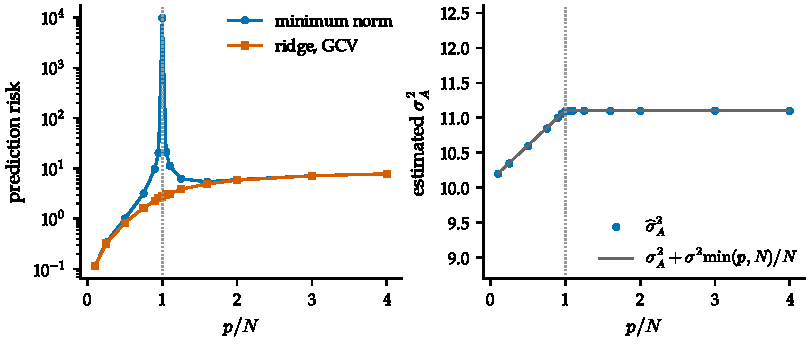
\includegraphics{figures/mp_dd.pdf}
\caption{$N=200$ individuals, ten causal variants of unit effect, sixty replicates. Left:
out of sample prediction risk on a logarithmic scale. The minimum norm interpolator peaks at
the interpolation threshold and descends beyond it; ridge with the scale chosen by
generalised cross validation is monotone and never spikes; at $p/N=4$ the two coincide at
$7.8$. Right: estimated $\sigma_A^2$ against $\sigma_A^2+\sigma^2\min(p,N)/N$, illustrating the
saturation of Corollary \ref{mp:cor:saturate}. The per point Monte Carlo standard error is
about $0.12$; the group means are $10.67$ below the threshold and $11.10$ at or above it,
against predictions of $10.68$ and $11.11$.}
\label{mp:fig:dd}
\end{figure}

The Bayesian reading of this, developed by \citet{mp:polson2025}, is the point we wish to
make here, and it bears directly on the assessment in the previous subsection. The
minimum norm solution is not assumption free. It is the posterior mean under a Gaussian prior
in the limit of infinite prior variance, restricted to the row space of $X$, and the peak at
$p=N$ is the divergence of that posterior as the smallest singular value approaches zero.
The descent beyond the threshold occurs because adding columns to a wide matrix raises its
smallest singular value, so the implicit prior is progressively better conditioned. Nothing
has been obtained for free; an assumption has been made silently and then rewarded.

Two consequences. First, the benign behaviour of the heavily overparameterised regime is
evidence about a particular implicit prior, not about overparameterisation as such. Second,
and visible in the left panel, an explicit prior removes the pathology entirely: the ridge
curve has no peak, and at $p/N=4$ it is indistinguishable from the interpolator. If one is
going to make an assumption in order to proceed, and Section \ref{mp:sec:overparam} argues that
one must, the argument for stating it is that a stated assumption can be tuned, criticised
and, in the case of Corollary \ref{mp:cor:singleton}, tested.

\section{Species sampling priors}
\label{mp:sec:kingman}

\subsection{Kingman's correspondence}

Let $\rho$ be a L\'evy density on $(0,\infty)$ with $\int_0^\infty\rho(x)\dd x=\infty$ and
$\int_0^\infty\min(1,x)\rho(x)\dd x<\infty$. Let $J_1\ge J_2\ge\cdots$ be the ranked points of a Poisson
process on $(0,\infty)$ with intensity $\rho$, put $T=\sum_iJ_i$, finite almost surely by
the second condition, and set
\begin{equation}
P_i \;=\; J_i/T,\qquad i=1,2,\dots
\label{mp:eq:normalise}
\end{equation}
\citet{mp:kingman1975} showed that \eqref{mp:eq:normalise} produces a random discrete
distribution and that drawing $n$ exchangeable samples from $(P_i)$ induces an exchangeable
random partition of $\{1,\dots,n\}$.

The two integrability conditions are worth separating, because they play opposite roles and
both are needed. The second, $\int_0^\infty\min(1,x)\rho(x)\dd x<\infty$, is what makes the
normalisation in \eqref{mp:eq:normalise} possible at all: its part on $(0,1)$ makes the small
jumps summable and its part on $(1,\infty)$ makes the large jumps finitely many, and without
it there is no
total to divide by. The first, $\int_0^\infty\rho(x)\dd x=\infty$, forces infinitely many
atoms, since the number of points exceeding $\varepsilon$ is Poisson with mean $\int_\varepsilon^\infty\rho(x)\dd x$, which tends to infinity as $\varepsilon\downarrow0$. It is the
formal expression of the statement that there are always more rare types waiting to be
discovered, and every result in this chapter about discovery rates is a quantitative refinement
of it.

Two cases are classical:
\[
\begin{gathered}
\rho(x)=\theta x^{-1}e^{-x}\ \Longrightarrow\ (P_i)\sim\PD(0,\theta),
\\
\rho(x)=\tfrac{\alpha}{\Gamma(1-\alpha)}x^{-1-\alpha}\ \Longrightarrow\
(P_i)\sim\PD(\alpha,0).
\end{gathered}
\]
The first is the gamma subordinator, for which the Laplace exponent is
$\psi(t)=\theta\log(1+t)$ and $T\sim\mathrm{Gamma}(\theta,1)$; the normalised jumps give the
Dirichlet process, and the total $T$ is independent of the normalised sequence $(P_i)$, a
special property of the gamma case which is what makes the Ewens Sampling Formula so
tractable. The second is the $\alpha$ stable subordinator, with $\psi(t)=t^\alpha$; here $T$
has no finite mean and is not independent of $(P_i)$, and that dependence is exactly what
Proposition \ref{mp:prop:fluct} later shows to be the source of the nonvanishing fluctuation in
the number of discovered types.

The relation between the two cases is the whole story. Both densities behave like a power of
$x$ near the origin, $x^{-1}$ in the first and $x^{-1-\alpha}$ in the second, and it is
behaviour near the origin that controls how many small atoms exist and hence how many rare
types a sample uncovers. The gamma case is the boundary $\alpha=0$ multiplied by the
exponential tilt $e^{-x}$, which is harmless at the origin but truncates the large jumps.
Corollary \ref{mp:cor:growth} below is, in the end, a statement about what that boundary costs: the pole $x^{-1}$, not the tilt,
converts a power law in the sample size into a logarithm, and no choice of $\theta$ recovers
the power.

\subsection{The Ewens Sampling Formula and its derivation from the subordinator}

The partition structure of $\PD(0,\theta)$ is the Ewens Sampling Formula
\citep{mp:ewens1972,mp:ewens2004}. For a sample of
$n$ genes with $a_j$ alleles represented exactly $j$ times, $\sum_jja_j=n$,
\begin{equation}
\Prob(a_1,\dots,a_n)=\frac{n!}{\theta_{(n)}}\prod_{j=1}^n\frac{1}{a_j!}
\Big(\frac{\theta}{j}\Big)^{a_j},\qquad
\theta_{(n)}=\frac{\Gamma(\theta+n)}{\Gamma(\theta)} ,
\label{mp:eq:esf}
\end{equation}
and equivalently, for a particular partition of $\{1,\dots,n\}$ into $k$ blocks of sizes $n_1,\dots,n_k$,
\begin{equation}
p(n_1,\dots,n_k\mid\theta)=\frac{\theta^k}{\theta_{(n)}}\prod_{i=1}^k(n_i-1)! .
\label{mp:eq:eppf}
\end{equation}

\begin{proposition}[Hoppe urn, \citealt{mp:hoppe1984}]
\label{mp:prop:hoppe}
Start with an urn containing a black ball of mass $\theta$. At each of $n$ steps draw a ball
with probability proportional to mass. If the black ball is drawn, return it together with a
new ball of a new colour and unit mass; otherwise return the drawn ball together with a
further ball of the same colour and unit mass. The colour partition of the $n$ draws has law
\eqref{mp:eq:eppf}.
\end{proposition}

Proposition \ref{mp:prop:hoppe} makes the formula simulable in $n$ steps and exhibits $\theta$
in its role as the rate at which new types appear. It is the source of the two facts we use
repeatedly: that $K_n$ is a sum of independent indicators, and that $\theta$ enters the
likelihood only through $K_n$.

\label{mp:sec:pk}

\medskip
\noindent\emph{From the subordinator to the sampling formula.} The correspondence of Section \ref{mp:sec:kingman} produces \eqref{mp:eq:eppf} explicitly, and the
calculation exhibits the exact point at which the exponential tilt enters. Define the Laplace exponent and the tilted moments of
$\rho$,
\[
\psi(t)=\int_0^\infty\big(1-e^{-tx}\big)\rho(x)\dd x,
\qquad
\xi(m,t)=\int_0^\infty x^m e^{-tx}\rho(x)\dd x .
\]

\begin{proposition}[Poisson Kingman partition formula]
\label{mp:prop:pk}
For the normalised subordinator \eqref{mp:eq:normalise}, the probability of a particular partition of $\{1,\dots,n\}$
into blocks of sizes $n_1,\dots,n_k$ summing to $n$ is
\begin{equation}
p(n_1,\dots,n_k)=\frac{1}{\Gamma(n)}\int_0^\infty t^{\,n-1}e^{-\psi(t)}
\prod_{i=1}^{k}\xi(n_i,t)\dd t .
\label{mp:eq:pkformula}
\end{equation}
\end{proposition}

\begin{example}[The gamma subordinator gives the Ewens Sampling Formula]
\label{mp:ex:gamma}
Take $\rho(x)=\theta x^{-1}e^{-x}$. Then
$\psi(t)=\theta\int_0^\infty(1-e^{-tx})x^{-1}e^{-x}\dd x=\theta\log(1+t)$ and
$\xi(m,t)=\theta\int_0^\infty x^{m-1}e^{-(1+t)x}\dd x=\theta\,\Gamma(m)(1+t)^{-m}$.
Substituting in \eqref{mp:eq:pkformula},
\[
\begin{aligned}
p(n_1,\dots,n_k)
&=\frac{\theta^{k}\prod_i(n_i-1)!}{\Gamma(n)}
\int_0^\infty t^{\,n-1}(1+t)^{-\theta-n}\dd t\\
&=\theta^{k}\prod_i(n_i-1)!\,\frac{B(n,\theta)}{\Gamma(n)}
=\frac{\theta^{k}}{\theta_{(n)}}\prod_i(n_i-1)! ,
\end{aligned}
\]
which is \eqref{mp:eq:eppf}.
\end{example}

\begin{example}[Kingman's correspondence at $n=3$]
\label{mp:ex:kingman3}
A sample of three genes can be partitioned in three ways up to labelling: all three alike,
written $(3)$; two alike and one different, $(2,1)$, which can happen in three labelled
ways; and all different, $(1,1,1)$. Proposition \ref{mp:prop:pk} gives the probability of
each labelled partition from the L\'evy density alone.

For the gamma subordinator with $\theta=2$ the formula of Example \ref{mp:ex:gamma} reads
$p(n_1,\dots,n_k)=2^k\prod_i(n_i-1)!/(2\cdot3\cdot4)$, so
\[
p(3)=\tfrac{2\cdot2}{24}=\tfrac16,\qquad
p(2,1)=\tfrac{4\cdot1}{24}=\tfrac16,\qquad
p(1,1,1)=\tfrac{8}{24}=\tfrac13 ,
\]
and $p(3)+3p(2,1)+p(1,1,1)=\tfrac16+\tfrac12+\tfrac13=1$, as it must.

For the stable subordinator, $\rho(x)=\alpha x^{-1-\alpha}/\Gamma(1-\alpha)$, the same
computation is a little longer and shows the tilt doing its work. Here $\psi(t)=t^\alpha$ and
$\xi(m,t)=\alpha\Gamma(m-\alpha)t^{\alpha-m}/\Gamma(1-\alpha)$, so the integrand in
\eqref{mp:eq:pkformula} is a power of $t$ times $e^{-t^\alpha}$, and the substitution
$u=t^\alpha$ gives $\int_0^\infty t^{k\alpha-1}e^{-t^\alpha}\dd t=\Gamma(k)/\alpha$. Hence
\[
p(n_1,\dots,n_k)=\frac{\alpha^{k-1}\,(k-1)!}{(n-1)!}\prod_{i=1}^k(1-\alpha)_{(n_i-1)} ,
\]
which is the two parameter formula \eqref{mp:eq:pyeppf} below at $\theta=0$. At
$\alpha=1/2$ and $n=3$,
\[
p(3)=\tfrac12\cdot\tfrac12\cdot\tfrac32=\tfrac38,\qquad
p(2,1)=\tfrac{\frac12\cdot1}{2}\cdot\tfrac12=\tfrac18,\qquad
p(1,1,1)=\tfrac{\frac14\cdot2}{2}=\tfrac14 ,
\]
again summing to one with the factor three on the middle term. The expected number of
alleles is $\E K_3=p(3)+6p(2,1)+3p(1,1,1)$, which is $13/6\approx2.167$ for the gamma case
with $\theta=2$ and $15/8=1.875$ for the stable case. Both values agree with the exact
formula \eqref{mp:eq:EKexact} below, and the integrals in \eqref{mp:eq:pkformula} were also
checked by numerical quadrature.

The stable case puts more mass on the extreme partitions $(3)$ and $(1,1,1)$ than a gamma
case with the same $\E K_3$ would: the gamma case with $\theta=1.092$ also has
$\E K_3=1.875$, but gives $p(3)=0.309$ and $p(1,1,1)=0.184$ against $0.375$ and $0.250$. That is the small sample face of the fluctuation result
of Section \ref{mp:sec:fluct}: a stable subordinator either has one dominant atom or many
small ones, and three genes are enough to see it.
\end{example}

Example \ref{mp:ex:gamma} shows where $\theta$ comes from and where the logarithm in
$\E K_n\sim\theta\log n$ comes from. The factor $\theta^k$ arises because
$\xi(m,t)$ carries one factor of $\theta$ per block, and the exponential tilt $e^{-x}$
in $\rho$ is what makes $\xi(m,t)$ decay like $(1+t)^{-m}$ rather than like a power of
$t$ alone. Replacing the simple pole $x^{-1}$ at the origin by $x^{-1-\alpha}$, with or without the tilt, replaces the
logarithm by $n^{\alpha}$, since the tilt is harmless at the origin. This is the mechanism behind Corollary \ref{mp:cor:growth}, stated
at the level of the L\'evy measure rather than at the level of the partition.

\subsection{The two families to be identified}

We now place side by side the two objects that Section \ref{mp:sec:main} identifies.

\medskip
\noindent\emph{Pitman's two parameter family.}

The two parameter family $\PD(\alpha,\theta)$, $0\le\alpha<1$, $\theta>-\alpha$, has
stick breaking representation $\GEM(\alpha,\theta)$,
\begin{equation}
W_1=V_1,\qquad W_i=V_i\prod_{j<i}(1-V_j),\qquad V_i\sim\Be(1-\alpha,\ \theta+i\alpha),
\label{mp:eq:gem}
\end{equation}
independently, and exchangeable partition probability function
\begin{equation}
p(n_1,\dots,n_k\mid\alpha,\theta)
=\frac{\prod_{i=1}^{k-1}(\theta+i\alpha)}{(\theta+1)_{(n-1)}}\prod_{i=1}^{k}(1-\alpha)_{(n_i-1)} ,
\label{mp:eq:pyeppf}
\end{equation}
where $x_{(m)}=x(x+1)\cdots(x+m-1)$ is the rising factorial, so that
$\theta_{(n)}=\theta\,(\theta+1)_{(n-1)}$. Setting $\alpha=0$ recovers \eqref{mp:eq:eppf}, and
the form with $(\theta+1)_{(n-1)}$ rather than $\theta_{(n)}$ in the denominator is the one that
remains meaningful at $\theta=0$. Dividing \eqref{mp:eq:pyeppf} for $n+1$ by its value for $n$
gives the predictive rule: given $k$ blocks of sizes $n_1,\dots,n_k$, the next draw joins
block $i$ with probability $(n_i-\alpha)/(\theta+n)$ and starts a new block with probability
$(\theta+k\alpha)/(\theta+n)$. The number of distinct blocks satisfies
\begin{equation}
\E K_n \sim
\begin{cases}
\dfrac{\Gamma(\theta+1)}{\alpha\Gamma(\theta+\alpha)}\,n^\alpha, & 0<\alpha<1,\\[8pt]
\theta\log n, & \alpha=0 .
\end{cases}
\label{mp:eq:Kn}
\end{equation}
In fact the mean is available exactly: for $0<\alpha<1$,
\begin{equation}
\E K_n=\frac{\Gamma(\theta+1)}{\alpha\,\Gamma(\theta+\alpha)}\,
\frac{\Gamma(\theta+\alpha+n)}{\Gamma(\theta+n)}-\frac{\theta}{\alpha},
\label{mp:eq:EKexact}
\end{equation}
and for $\alpha=0$, $\E K_n=\sum_{j=0}^{n-1}\theta/(\theta+j)$; both are proved in Section
\ref{mp:app:proofs}, and the asymptotics \eqref{mp:eq:Kn} follow from
$\Gamma(x+\alpha)/\Gamma(x)\sim x^\alpha$.
The dichotomy in \eqref{mp:eq:Kn} is the whole story of what follows. A positive $\alpha$ gives
a power law in the sample size; $\alpha=0$ gives a logarithm, however large $\theta$ is
made.

\medskip
\noindent\emph{Global local shrinkage priors.} A global local prior for a many parameter
mean vector is
\begin{equation}
\beta_i\mid\lambda_i,\tau\sim N(0,\tau^2\lambda_i^2),\qquad \lambda_i\sim\pi(\lambda),
\label{mp:eq:gl}
\end{equation}
and with unit observation variance the shrinkage weight is
$\kappa_i=1/(1+\tau^2\lambda_i^2)$, so that $\E(\beta_i\mid y_i)=(1-\E(\kappa_i\mid y_i))y_i$
and $\kappa_i=1$ is total shrinkage while $\kappa_i=0$ is none. The standard family is the
three parameter beta normal class of \citet{mp:armagan2011}, in which
$\kappa\sim\Be(a,b)$ with $a\in(0,1]$, $b>0$, the density being
$f_\kappa(x)=x^{a-1}(1-x)^{b-1}/B(a,b)$. The exponent $a$ governs the behaviour near
$\kappa=0$, that is how readily large effects escape shrinkage, and $b$ the behaviour near
$\kappa=1$, how hard small effects are pulled to zero. The horseshoe of
\citet{mp:carvalho2010} is $a=b=1/2$, the arcsine law, with poles at both ends. The prior of
\citet{mp:strawderman1971} and \citet{mp:berger1980} is $(a,b)=(1/2,1)$, with the pole at
zero but none at one. The uniform shrinkage prior, $\kappa$ uniform on $(0,1)$, is
$a=b=1$ and has no pole at all.

\citet{mp:polson2012} showed that \eqref{mp:eq:gl} is generated by the increments of a
subordinator, the object that Kingman's construction normalises. It is therefore unsurprising that the two
families should be related. What is perhaps surprising is that the relation is an identity.

\section{Sparsity level is Pitman's alpha}
\label{mp:sec:main}

This section proves that the two families of Section \ref{mp:sec:kingman} are linked by an exact identity of marginal laws. The idea
is simple. A shrinkage weight $\kappa$ near zero means an effect left almost untouched, and
under a species sampling prior a stick breaking weight near zero means a rare type; both
families have a single parameter, $a$ on one side and $\alpha$ on the other, that controls
how much mass the law places near zero. Matching those two parameters, and then the second
parameter on each side, gives an exact identity.

\begin{theorem}[Shrinkage weights are stick breaking weights]
\label{mp:thm:main}
Let $\kappa\sim\Be(a,b)$ with $a\in(0,1]$ and $b>0$. Then $\kappa$ has the law of the first
stick breaking weight $W_1$ of $\GEM(\alpha,\theta)$ in \eqref{mp:eq:gem} under
\[
\alpha=1-a,\qquad \theta=a+b-1,
\]
and this map is a bijection from $\{a\in(0,1],\ b>0\}$ onto
$\{0\le\alpha<1,\ \theta>-\alpha\}$.
\end{theorem}

Matching parameters in \eqref{mp:eq:gem} gives $1-\alpha=a$ and $\theta+\alpha=b$; that the map
is onto is checked in Section \ref{mp:app:proofs}.

\begin{corollary}
\label{mp:cor:cases}
The horseshoe, $\kappa\sim\Be(1/2,1/2)$, corresponds to $(\alpha,\theta)=(1/2,0)$, that is
to $\PD(1/2,0)$, the normalised one half stable subordinator. The Strawderman Berger prior,
$\kappa\sim\Be(1/2,1)$, corresponds to $(\alpha,\theta)=(1/2,1/2)$. The uniform shrinkage
prior, $\kappa\sim\Be(1,1)$, corresponds to $(\alpha,\theta)=(0,1)$, that is to the Dirichlet
process with $\theta=1$, whose partition structure is \eqref{mp:eq:esf} at $\theta=1$.
\end{corollary}

The arcsine law that gives the horseshoe its name is therefore not an algebraic convenience.
It is the signature of $\alpha=1/2$, and the same law appears in L\'evy's arcsine theorem
for Brownian motion for the same reason, the one half stable subordinator being the inverse
of Brownian local time. Table \ref{mp:tab:dict} lists the priors of this chapter with their pairs $(\alpha,\theta)$ and the order of $\E K_n$.

\begin{table}[t]
\centering
\begin{adjustbox}{max width=\textwidth}
\begin{tabular}{lccc}
\toprule
prior & $\kappa\sim$ & $(\alpha,\theta)$ & $\E K_n$ \\
\midrule
horseshoe & $\Be(1/2,1/2)$ & $(1/2,\ 0)$ & $\asymp n^{1/2}$ \\
three parameter beta, general & $\Be(a,b)$ & $(1-a,\ a+b-1)$ & $\asymp n^{1-a}$ \\
Strawderman Berger & $\Be(1/2,1)$ & $(1/2,\ 1/2)$ & $\asymp n^{1/2}$ \\
uniform shrinkage & $\Be(1,1)$ & $(0,\ 1)$ & $\asymp\log n$ \\
ridge like, $b>1$ & $\Be(1,b)$ & $(0,\ b)$ & $\asymp b\log n$ \\
Bayesian lasso, normal gamma & no pole at $\kappa=0$ & $\alpha=0$ & $\asymp\log n$ \\
\bottomrule
\end{tabular}
\end{adjustbox}
\caption{The dictionary of Theorem \ref{mp:thm:main}. The final row is an application neither of
the theorem nor of Corollary \ref{mp:cor:growth}: it reads these priors through the gamma
subordinator, an $\alpha=0$ object with $\E K_n\sim\theta\log n$. Used directly at
$\tau_n=n^{-1/2}$ their effective model size is bounded (see the paragraph after Corollary
\ref{mp:cor:growth}), so for them $\log n$ is an upper bound only. The horseshoe plus and Dirichlet Laplace
priors are outside the $\Be(a,b)$ family and are not covered by the table.}
\label{mp:tab:dict}
\end{table}

\subsection{Consequences: the frequency spectrum and the discovery rate}

Theorem \ref{mp:thm:main} is an identity for a single weight. The following extends the identification from one
weight to the mean intensity of the entire spectrum, and is the result on which the genetic reading of the chapter
rests.

Theorem \ref{mp:thm:main} identifies $\kappa$ with the first stick breaking weight $W_1$, and
what the next result needs is a size biased pick. These are the same object, by a classical
theorem of Pitman which we record because the identification is the hinge of the argument.

\begin{lemma}[Stick breaking is size biased]
\label{mp:lem:sizebias}
The sequence $(W_i)$ of \eqref{mp:eq:gem} is the size biased permutation of the ranked
frequencies of $\PD(\alpha,\theta)$. In particular $W_1$ is a size biased pick, that is
$\Prob(W_1\in A)=\E\sum_i P_i\mathbf 1(P_i\in A)$.
\end{lemma}

Lemma \ref{mp:lem:sizebias} is Pitman's residual allocation result \citep{mp:pitman1996,mp:pitmanyor1997}
and we do not reprove it. Its
consequence here is that the density of $\kappa$ supplied by Theorem \ref{mp:thm:main} is the
density of a size biased pick, which is exactly the input required below.

\begin{theorem}[Spectrum and shrinkage profile]
\label{mp:thm:spectrum}
Let $(P_i)$ be a random discrete distribution and let $\nu$ be the mean intensity of its
atoms, so that $\E\sum_ih(P_i)=\int_0^1h(x)\nu(x)\dd x$ for bounded $h$ vanishing at the
origin. Let $W$ be a size biased pick from $(P_i)$, with density $f_W$. Then
\[
f_W(x)=x\,\nu(x),\qquad\text{equivalently}\qquad \nu(x)=x^{-1}f_W(x).
\]
Consequently, for a global local prior whose shrinkage weight density $f_\kappa$ is matched
by Theorem \ref{mp:thm:main}, so that $f_\kappa=f_W$ by Lemma \ref{mp:lem:sizebias}, the induced
allele frequency spectrum satisfies
\begin{equation}
\E\,a_j=\binom{n}{j}\int_0^1x^{j-1}(1-x)^{n-j}f_\kappa(x)\dd x .
\label{mp:eq:aj}
\end{equation}
\end{theorem}

\begin{corollary}[Fisher's log series]
\label{mp:cor:logseries}
For $\kappa\sim\Be(1,\theta)$, that is $(\alpha,\theta)=(0,\theta)$, \eqref{mp:eq:aj} gives
\[
\E a_j=\frac{\theta}{j}\cdot\frac{n!}{(n-j)!}\cdot
\frac{\Gamma(\theta+n-j)}{\Gamma(\theta+n)}\ \longrightarrow\ \frac{\theta}{j}
\]
as $n\to\infty$ with $j$ fixed, which is Fisher's log series and the expected frequency
spectrum of the Ewens Sampling Formula.
\end{corollary}

\begin{corollary}[Singletons under the horseshoe]
\label{mp:cor:singleton}
For the horseshoe, $f_\kappa(x)=\{\pi\sqrt{x(1-x)}\}^{-1}$, \eqref{mp:eq:aj} at $j=1$ gives
$\E a_1=n\,B(1/2,n-1/2)/\pi\sim\sqrt{n/\pi}$.
\end{corollary}

\begin{example}[Two spectra with the same number of alleles]
\label{mp:ex:spectra}
Take $n=20$ genes and compare the Ewens Sampling Formula at $\theta=2$, that is
$\kappa\sim\Be(1,2)$, with the horseshoe, $\PD(1/2,0)$. Their expected numbers of alleles are
close, $5.29$ and $5.01$, but \eqref{mp:eq:aj} shows the alleles are spread differently:
\begin{center}
\begin{tabular}{lrrrrrr}
\toprule
$j$ & $1$ & $2$ & $3$ & $4$ & $5$ & $6$ \\
\midrule
Ewens, $\theta=2$ & $1.905$ & $0.905$ & $0.571$ & $0.405$ & $0.305$ & $0.238$ \\
log series $\theta/j$ & $2.000$ & $1.000$ & $0.667$ & $0.500$ & $0.400$ & $0.333$ \\
horseshoe, $\PD(1/2,0)$ & $2.572$ & $0.660$ & $0.340$ & $0.219$ & $0.158$ & $0.123$ \\
\bottomrule
\end{tabular}
\end{center}
The first entry can be checked by hand: Corollary \ref{mp:cor:logseries} at $j=1$ gives
$\E a_1=\theta n/(\theta+n-1)=40/21=1.905$. In both cases $\sum_jj\,\E a_j=20$, as it must,
since every gene belongs to exactly one allele. The horseshoe spectrum is more top heavy
at both ends: more singletons, and more of the sample concentrated in one or two common
alleles, with a thinner middle. With only twenty genes the log series is still a rough
guide to the Ewens means, and the convergence in Corollary \ref{mp:cor:logseries} is visibly
slow at larger $j$, where the factor $n!\,\Gamma(\theta+n-j)/\{(n-j)!\,\Gamma(\theta+n)\}$
is furthest from one.
\end{example}

Corollary \ref{mp:cor:singleton} is a sharp consistency check, not merely a plausibility one.
Under $\PD(1/2,0)$, \eqref{mp:eq:Kn} gives $\E K_n\sim\Gamma(1)n^{1/2}/\{\tfrac12\Gamma(\tfrac12)\}
=1.128\,n^{1/2}$, while Corollary \ref{mp:cor:singleton} gives
$\E a_1\sim\sqrt{n/\pi}=0.564\,n^{1/2}$. The ratio is exactly $1/2$. That is the value
required by the general fact that under $\PD(\alpha,\theta)$ with $\alpha>0$ the proportion of
blocks of size $j$ converges to $\alpha(1-\alpha)_{(j-1)}/j!$, which at $j=1$ is $\alpha$
\citep{mp:pitman2006}. Three independently derived quantities, the spectrum formula
\eqref{mp:eq:aj}, the growth rate \eqref{mp:eq:Kn} and the singleton fraction, therefore agree.
(On the shrinkage side Theorem \ref{mp:thm:effsize} gives the constant $1$ rather than $1.128$,
the factor $\Gamma(3/2)=0.886$ of Corollary \ref{mp:cor:agree}.) It is also a statement about rare variant discovery with a direct
empirical content. An $\alpha=1/2$ prior expects the number of singleton variants to grow
as the square root of the sample size; an $\alpha=0$ prior expects it to converge to
$\theta$. These are different biological claims about the same data, and modern sequencing
studies, in which singletons dominate the discovered spectrum, appear to favour the former.

\medskip
\noindent\emph{Discovery rates.}

\begin{corollary}[Discovery rates]
\label{mp:cor:growth}
Under Theorem \ref{mp:thm:main} and \eqref{mp:eq:Kn}, a global local prior with
$\kappa\sim\Be(a,b)$ induces an expected number of occupied blocks in a sample of size $n$
growing like $n^{1-a}$ when $a<1$ and like $(a+b-1)\log n$ when $a=1$. In particular the
horseshoe discovers of the order of $n^{1/2}$ signals, and every prior with $a=1$, that is
the uniform shrinkage prior and the ridge like priors $\Be(1,b)$, discovers of the order of
$b\log n$.
\end{corollary}

Laplace type priors such as the Bayesian lasso are not covered by Corollary
\ref{mp:cor:growth}, because they are not in the $\Be(a,b)$ family: with $\lambda^2$
exponential, the density of $\kappa$ vanishes at the origin faster than any power, so no
finite $a$ matches it. The last row of Table \ref{mp:tab:dict} reads such priors through
their species sampling counterpart, the gamma subordinator, which is the boundary
$\alpha=0$ with $\E K_n\sim\theta\log n$. Used directly, with independent local scales at
$\tau_n=n^{-1/2}$, the same priors have a bounded effective model size: the expected value
of \eqref{mp:eq:effsize} tends to $\E\lambda^2$, and with $\lambda^2$ exponential of mean one
it is $0.981$ at $n=10^2$ and $1.000$ at $n=10^6$, against $\log n=4.61$ and $13.82$. For
them $\log n$ is therefore an upper bound, not a rate.

The reading in the last row of Table \ref{mp:tab:dict} is, to our knowledge, a new explanation of a well documented
empirical phenomenon. It is standard that the lasso underselects in the ultra sparse regime
while the horseshoe does not, and the usual explanation is in terms of tail thickness and
minimax risk. The explanation here is Kingman's: a L\'evy density that behaves like $x^{-1}$ at the origin, as that of the gamma subordinator does, is an $\alpha=0$ object, and an $\alpha=0$ object cannot discover more than logarithmically many species however many are present. The exponential tilt is not the point, since it only tames the large jumps and equals one at the origin; what matters is the order of the pole of the L\'evy density at the origin, which is where the rare types live. The lesson transfers back to genetics unchanged: a prior on effect sizes whose L\'evy density has a simple pole at the origin is a prior which asserts, before seeing any
data, that the number of contributing variants is logarithmic in the sample.

\subsection{The rate holds for the shrinkage prior itself}
\label{mp:sec:direct}

Corollary \ref{mp:cor:growth} is a statement about the matched species sampling model, and a
reader is entitled to ask whether it says anything about the prior \eqref{mp:eq:gl} as actually
used, in which the weights are independent across coordinates rather than sampled from a
normalised subordinator. It does, and the following makes the statement directly, without
passing through the partition.

The natural count on the shrinkage side is the effective model size
\begin{equation}
m_p \;=\; \sum_{i=1}^{p}(1-\kappa_i),
\label{mp:eq:effsize}
\end{equation}
the sum of the fractions of the weighted least squares coefficients \eqref{mp:eq:kappaWLS} that
survive the penalty. It is the shrinkage analogue of $K_n$, and it is the quantity the
horseshoe literature reports as the effective number of parameters.

\begin{theorem}[Effective model size]
\label{mp:thm:effsize}
Let $\kappa_\tau=1/(1+\tau^2\lambda^2)$ where $\lambda$ is such that $\kappa_1\sim\Be(a,b)$
with $a\in(0,1]$, $b>0$. Then as $\tau\downarrow0$
\[
\E(1-\kappa_\tau)\;\sim\;
\begin{cases}
\dfrac{\pi}{B(a,b)\sin(\pi a)}\ \tau^{2a}, & 0<a<1,\\[8pt]
2b\,\tau^{2}\log(1/\tau), & a=1 .
\end{cases}
\]
Consequently, for $p=n$ coordinates at the canonical global scale $\tau_n=n^{-1/2}$,
\[
\E\,m_n \;\sim\;
\begin{cases}
\dfrac{\pi}{B(a,b)\sin(\pi a)}\ n^{1-a}, & 0<a<1,\\[8pt]
b\log n, & a=1 .
\end{cases}
\]
\end{theorem}

\begin{corollary}[The rates agree, and the constants nearly do]
\label{mp:cor:agree}
The rates in Theorem \ref{mp:thm:effsize} are exactly those of $\E K_n$ under
$\PD(\alpha,\theta)$ with $(\alpha,\theta)=(1-a,\ a+b-1)$, that is under the matching of
Theorem \ref{mp:thm:main}. The constants agree exactly when $a=1$, both being $b$, and for
$a<1$ they differ by the factor $\Gamma(2-a)$, which lies in
$[\Gamma(1.4616),1]\approx[0.8856,1]$ for every $a\in(0,1]$.
\end{corollary}

Theorem \ref{mp:thm:effsize} and Corollary \ref{mp:cor:agree} are, in our view, the results that
make the chapter more than a translation. They say that the global local prior in its ordinary
form, with independent local scales and the standard global scale $\tau_n=n^{-1/2}$, produces
the discovery rate of the matched Poisson Dirichlet process, with the same exponent and a
constant agreeing to within twelve per cent uniformly in $a$. Nothing in the derivation uses
the partition structure. The exponent $2a$ in Theorem \ref{mp:thm:effsize} arises from the
behaviour of the beta prime density at the origin, and $1-a$ appears in $\E K_n$ because
$\alpha=1-a$; that these produce the same power of $n$ at $\tau_n=n^{-1/2}$ is what has to
be checked, and it is what the theorem checks.

It also explains a convention. The choice $\tau_n=n^{-1/2}$ is standard in the horseshoe
literature and is usually justified by risk considerations. Theorem \ref{mp:thm:effsize} gives a
second reading: it is the unique power of $n$ at which the effective model size reproduces
the species sampling discovery rate for every $a$ simultaneously. At any other power the two
sides disagree, and they disagree differently for different $a$.

\begin{table}[t]
\centering
\begin{adjustbox}{max width=\textwidth}
\begin{tabular}{lrrrrr}
\toprule
$(a,b)$ & $(\alpha,\theta)$ & $n=10^3$ & $n=10^4$ & $n=10^5$ & predicted at $n=10^5$ \\
\midrule
$(1/2,1/2)$ horseshoe & $(1/2,0)$ & $30.65$ & $99.01$ & $315.23$ & $316.23$ \\
$(1,1)$ uniform shrinkage & $(0,1)$ & $5.92$ & $8.21$ & $10.51$ & $11.51$ \\
$(1,3)$ & $(0,3)$ & $15.29$ & $22.14$ & $29.04$ & $34.54$ \\
\bottomrule
\end{tabular}
\end{adjustbox}
\caption{Expected effective model size $\E m_n$ of \eqref{mp:eq:effsize} at
$\tau_n=n^{-1/2}$, computed by numerical quadrature of the one dimensional integral in the
proof of Theorem \ref{mp:thm:effsize}, against the leading term of that theorem. The horseshoe
row is $n^{1/2}$ to within $0.4$ per cent at $n=10^5$; the two rows with $a=1$ grow by
$b\log 10$ per decade, that is by $2.30$ and $6.91$, against computed increments of $2.29$
and $2.30$, and $6.85$ and $6.90$.}
\label{mp:tab:effsize}
\end{table}

Table \ref{mp:tab:effsize} evaluates both sides. The horseshoe attains $315.23$ against the
predicted $\sqrt{10^5}=316.23$, and the two priors with $a=1$ increase by a fixed amount per
decade of $n$, which is the signature of logarithmic growth. The finite $n$ agreement is
better for $a<1$ than for $a=1$, as it should be, since the logarithmic case carries a
relative correction of order $1/\log(1/\tau)$.

\begin{example}[Three members of the beta normal class, side by side]
\label{mp:ex:tpb}
Take the horseshoe $(a,b)=(1/2,1/2)$, the uniform shrinkage prior $(1,1)$ and the
Strawderman Berger prior $(1/2,1)$. Theorem \ref{mp:thm:main} sends them to
$\GEM(1/2,0)$, $\GEM(0,1)$ and $\GEM(1/2,1/2)$ respectively, and Theorem
\ref{mp:thm:spectrum} gives the frequency spectrum intensities
\[
\nu_{\mathrm{HS}}(x)=\frac{1}{\pi}\,x^{-3/2}(1-x)^{-1/2},\qquad
\nu_{\mathrm{U}}(x)=x^{-1},\qquad
\nu_{\mathrm{SB}}(x)=\tfrac12\,x^{-3/2},
\]
on $0<x<1$, the constants being $1/B(a,b)$, namely $1/\pi$, $1$ and $1/B(\tfrac12,1)=\tfrac12$.
The power of $x$ at the origin is $a-2$: it is $x^{-3/2}$ for both priors with $a=1/2$, which
is what makes their discovery counts grow like $n^{1/2}$, and $x^{-1}$ for the uniform prior,
which is the borderline case giving a logarithm. The two $a=1/2$ priors differ only near
$x=1$, that is in how they treat common alleles, and this changes the level of the discovery
curve but not its rate.

Table \ref{mp:tab:tpb} evaluates four quantities at $n=10^2$, $10^3$ and $10^4$: the exact
$\E K_n$ from \eqref{mp:eq:EKexact}, its leading term from \eqref{mp:eq:Kn}, the expected
number of singletons $\E a_1=n\,B(a,b+n-1)/B(a,b)$ from \eqref{mp:eq:aj}, and the expected
effective model size $\E m_n$ of \eqref{mp:eq:effsize} at $\tau_n=n^{-1/2}$, computed by
quadrature. Several entries can be checked by hand. For the uniform prior $\E K_n$ is the
harmonic number $\sum_{j=1}^n j^{-1}$, which is $5.187$ at $n=100$, and $\E a_1=n\,B(1,n)=1$
exactly, for every $n$: under the Ewens Sampling Formula with $\theta=1$ one expects a single
singleton however large the sample. For the horseshoe \eqref{mp:eq:EKexact} reduces to
$\E K_n=2\Gamma(n+\tfrac12)/\{\sqrt\pi\,\Gamma(n)\}$, which at $n=100$ is
$1.1284\times\sqrt{100}\times(1-1/800)=11.27$ to four figures.

\begin{table}[t]
\centering
\begin{adjustbox}{max width=\textwidth}
\begin{tabular}{llrrrr}
\toprule
prior, $(\alpha,\theta)$ & $n$ & $\E K_n$ & leading term & $\E a_1$ & $\E m_n$ \\
\midrule
horseshoe, $(1/2,0)$ & $10^2$ & $11.27$ & $11.28$ & $5.66$ & $9.09$ \\
 & $10^3$ & $35.68$ & $35.68$ & $17.85$ & $30.65$ \\
 & $10^4$ & $112.84$ & $112.84$ & $56.42$ & $99.01$ \\
\midrule
uniform, $(0,1)$ & $10^2$ & $5.19$ & $4.61$ & $1.00$ & $3.69$ \\
 & $10^3$ & $7.49$ & $6.91$ & $1.00$ & $5.92$ \\
 & $10^4$ & $9.79$ & $9.21$ & $1.00$ & $8.21$ \\
\midrule
Strawderman Berger, $(1/2,1/2)$ & $10^2$ & $16.75$ & $17.72$ & $8.87$ & $13.92$ \\
 & $10^3$ & $55.06$ & $56.05$ & $28.03$ & $47.74$ \\
 & $10^4$ & $176.25$ & $177.25$ & $88.62$ & $155.10$ \\
\bottomrule
\end{tabular}
\end{adjustbox}
\caption{Discovery counts for three members of the three parameter beta normal class.
$\E K_n$ is exact, from \eqref{mp:eq:EKexact}; the leading term is $1.128\,n^{1/2}$,
$\log n$ and $\sqrt\pi\,n^{1/2}=1.772\,n^{1/2}$ respectively; $\E a_1$ is the expected number
of singletons from \eqref{mp:eq:aj}; $\E m_n$ is the expected effective model size of the
shrinkage prior at $\tau_n=n^{-1/2}$, whose leading terms by Theorem \ref{mp:thm:effsize} are
$n^{1/2}$, $\log n$ and $(\pi/2)n^{1/2}$.}
\label{mp:tab:tpb}
\end{table}

Three things are visible in the table. First, the two $a=1/2$ priors multiply their
discoveries by $\sqrt{10}\approx3.16$ per decade of $n$, while the uniform prior adds
$\log10\approx2.30$ per decade; by $n=10^4$ the Strawderman Berger prior expects $176$ alleles
and the uniform prior fewer than ten. Second, the singleton fraction $\E a_1/\E K_n$ is
$0.500$ for the horseshoe and $0.503$ for the Strawderman Berger prior at $n=10^4$, both close
to $\alpha=1/2$, while for the uniform prior it is $1/9.79=0.10$ and falling towards zero; the
singleton fraction therefore separates $\alpha$ even when the levels are matched. Third, the
effective model size of the shrinkage prior tracks $\E K_n$ with ratio $0.88$ for both
$a=1/2$ priors at $n=10^4$, close to $\Gamma(3/2)=0.886$, exactly as Corollary
\ref{mp:cor:agree} predicts; for the uniform prior the ratio $8.21/9.79=0.84$ is still
converging to one at the slow logarithmic rate.
\end{example}

\subsection{Where the correspondence stops: fluctuations}
\label{mp:sec:fluct}

Theorem \ref{mp:thm:effsize} matches first moments. It is worth asking whether the agreement
extends to second moments, and the answer is that it does not. The failure is instructive,
because it says exactly what the unproved partition identity would buy.

\begin{lemma}[Second moment]
\label{mp:lem:second}
Under the hypotheses of Theorem \ref{mp:thm:effsize} with $0<a<1$,
\[
\E(1-\kappa_\tau)^2 \;\sim\; \frac{B(a,2-a)}{B(a,b)}\,\tau^{2a}
\qquad\text{as }\tau\downarrow0 ,
\]
so that $\Var(1-\kappa_\tau)\sim\{B(a,2-a)/B(a,b)\}\tau^{2a}$, the square of the mean being
of the smaller order $\tau^{4a}$.
\end{lemma}

\begin{proposition}[The two constructions fluctuate differently]
\label{mp:prop:fluct}
Fix $a\in(0,1)$ and $b>0$, let $\kappa_1,\dots,\kappa_n$ be independent with the law of
$\kappa_{\tau_n}$ at $\tau_n=n^{-1/2}$, put $m_n=\sum_{i=1}^n(1-\kappa_i)$, and let $K_n$ be
the number of blocks in a sample of size $n$ from $\PD(\alpha,0)$ with $\alpha=1-a$. Then
\[
\begin{gathered}
\frac{m_n}{\E m_n}\ \xrightarrow{\ \Prob\ }\ 1,
\qquad\text{with}\\
\frac{\{\Var m_n\}^{1/2}}{\E m_n}\ \sim\ \frac{\sin(\pi a)}{\pi}\big\{B(a,2-a)\,B(a,b)\big\}^{1/2}\, n^{-(1-a)/2},
\end{gathered}
\]
whereas $K_n/n^{\alpha}\to M_\alpha$ almost surely, where $M_\alpha$ is Mittag Leffler with
$\E M_\alpha^r=r!/\Gamma(1+r\alpha)$. The limit is nondegenerate, so the coefficient of
variation of $K_n$ converges to
$\{2\Gamma(1+\alpha)^2/\Gamma(1+2\alpha)-1\}^{1/2}$, equal to $0.7555$ at $\alpha=1/2$,
while that of $m_n$ converges to zero.
\end{proposition}

\begin{proof}
By Lemma \ref{mp:lem:second} and Theorem \ref{mp:thm:effsize},
$\Var m_n = n\Var(1-\kappa_{\tau_n})\sim\{B(a,2-a)/B(a,b)\}n^{1-a}$ and
$\E m_n\sim\{\pi/(B(a,b)\sin\pi a)\}n^{1-a}$, so with $C_2=B(a,2-a)/B(a,b)$ and $C_1=\pi/\{B(a,b)\sin(\pi a)\}$ the ratio of standard
deviation to mean is $C_2^{1/2}C_1^{-1}n^{-1/2}\tau_n^{-a}=C_2^{1/2}C_1^{-1}n^{-(1-a)/2}$,
and $C_2^{1/2}/C_1=\{B(a,2-a)B(a,b)\}^{1/2}\sin(\pi a)/\pi$. Chebyshev then gives convergence
in probability, since the ratio tends to zero for every $a<1$. The
statement for $K_n$ is Pitman's almost sure limit theorem for the two parameter family, and
the moments of $M_\alpha$ are classical.
\end{proof}

Table \ref{mp:tab:fluct} confirms both.

\begin{table}[t]
\centering
\begin{adjustbox}{max width=\textwidth}
\begin{tabular}{lrrrrrr}
\toprule
& \multicolumn{3}{c}{$K_n$ under $\PD(1/2,0)$} & \multicolumn{3}{c}{$m_n$, horseshoe at $\tau_n=n^{-1/2}$} \\
\cmidrule(lr){2-4}\cmidrule(lr){5-7}
$n$ & mean & s.d. & c.v. & mean & s.d. & c.v. \\
\midrule
$200$   & $15.91$ & $11.86$ & $0.745$ & $13.20$ & $2.53$ & $0.192$ \\
$1000$  & $35.36$ & $25.57$ & $0.723$ & $30.56$ & $3.86$ & $0.126$ \\
$5000$  & $76.66$ & $57.87$ & $0.755$ & $69.51$ & $6.01$ & $0.086$ \\
\bottomrule
\end{tabular}
\end{adjustbox}
\caption{Four hundred replicates at each $n$. The means agree to within the factor
$\Gamma(2-a)$ of Corollary \ref{mp:cor:agree}, as they should. The coefficients of variation do
not. That of $K_n$ stays near the Mittag Leffler value $0.7555$ at every $n$, while that of
$m_n$ decays: the fitted exponent across the three sample sizes is $-0.250$ against the
predicted $-1/4$. The closed form prediction of Proposition \ref{mp:prop:fluct}, which at $a=b=1/2$ has constant
$2^{-1/2}$ and so gives $0.188$, $0.126$ and $0.084$, agrees with the simulated values to within the Monte Carlo error of a coefficient of variation estimated from four
hundred replicates, which is about four per cent.}
\label{mp:tab:fluct}
\end{table}

The reason is dependence. Under $\PD(\alpha,0)$ the atom frequencies are the normalised jumps
of an $\alpha$ stable subordinator, whose total is itself heavy tailed, so a sample either
lands in a realisation with many large atoms or in one with few, and that randomness never
averages away. The independent weights of \eqref{mp:eq:gl} have no such common factor and obey
a law of large numbers.

We regard this as clarifying rather than damaging. Corollary \ref{mp:cor:growth} is a statement
about how many signals a prior expects to find, and Theorem \ref{mp:thm:effsize} establishes it
for the prior as used. What Proposition \ref{mp:prop:fluct} shows is that the correspondence is
one of means and not of laws, and that a practitioner who wants a prior which is genuinely
uncertain about the number of signals, rather than merely uncertain about which ones, must
introduce the dependence explicitly, for instance by estimating $\tau$ rather than fixing it.
That is the practical content of the open problem in the remark below: the partition identity,
if true, would settle whether estimating $\tau$ is the device which supplies the missing
common factor.

\begin{remark}[What is and is not proved]
\label{mp:rem:open}
Theorems \ref{mp:thm:main} and \ref{mp:thm:spectrum} concern the random discrete distribution
generated by a normalised subordinator, whereas \eqref{mp:eq:gl} places independent weights on a
fixed index set. We have not shown that the exchangeable partition induced on coefficient
indices by \eqref{mp:eq:gl} coincides with the $\PD(\alpha,\theta)$ partition, and we do not
claim it.

What Theorem \ref{mp:thm:effsize} shows is that the consequence which matters, namely the
discovery rate, transfers without that identification. The rate is derived directly from the
law of $\kappa$ under \eqref{mp:eq:gl} and agrees with the species sampling rate in exponent
exactly and in constant to within $\Gamma(2-a)$. So Corollary \ref{mp:cor:growth} may be read as
a statement about the shrinkage prior as used, and Theorem \ref{mp:thm:main} may be read as the
explanation of why that rate takes the form it does rather than as a premise the rate depends
on.

The partition level identity remains open and would still be worth having, and Proposition
\ref{mp:prop:fluct} says precisely why: the correspondence established here is one of first
moments, and the two constructions differ at second order, the species sampling side
retaining a nonvanishing coefficient of variation which the independent weights side does
not. A partition level identity would settle whether estimating the global scale supplies the
missing dependence.
\end{remark}

\section{Inference for the mutation parameter}
\label{mp:sec:conj}

By Corollary \ref{mp:cor:cases}, $\theta$ is the parameter fixing how many discoveries the
prior expects. It is therefore worth inferring rather than fixing. This section collects the
three facts that make inference about $\theta$ easy in principle and hard in practice:
the likelihood depends on the data only through the number of alleles, that number is a sum
of independent Bernoulli variables, and the awkward ratio of gamma functions in the
likelihood can be removed by one latent beta variable per locus. Worked examples on a small
sample, on several loci and on a classical ecological data set follow.

\begin{proposition}[\citealt{mp:ewens1972}]
\label{mp:prop:suff}
Under \eqref{mp:eq:eppf} the number of distinct alleles $K_n$ is sufficient for $\theta$, and
it is minimal sufficient.
\end{proposition}

\begin{proof}
Write \eqref{mp:eq:eppf} as $h(\pi)g(K_n(\pi),\theta)$ with $h(\pi)=\prod_i(n_i-1)!$ and
$g(k,\theta)=\theta^k/\theta_{(n)}$; Fisher Neyman gives sufficiency. For two partitions of
the same $n$, $p(\pi\mid\theta)/p(\pi'\mid\theta)=\{h(\pi)/h(\pi')\}\theta^{K_n(\pi)-K_n(\pi')}$
is free of $\theta$ if and only if $K_n(\pi)=K_n(\pi')$, so by the Lehmann Scheff\'e
criterion $K_n$ is minimal sufficient.
\end{proof}

In the terms of \citet{mp:edwards1972}, the content of Proposition \ref{mp:prop:suff} is that the
likelihood function for $\theta$, considered as a function on the parameter space, is
determined up to a multiplicative constant by the single integer $K_n$: the entire allelic
configuration, which for $n=1000$ genes may specify a partition of enormous complexity,
carries no further information about the mutation parameter. This is an unusually clean
instance of the reduction that Edwards takes to be the central object of inference, and it is
what makes the model the natural place to test any procedure that claims to find such
reductions automatically.

\begin{proposition}[Feller coupling]
\label{mp:prop:feller}
$K_n$ has the law of $\sum_{j=0}^{n-1}B_j$ with $B_j$ independent Bernoulli of success
probability $\theta/(\theta+j)$. Hence
$\E K_n=\sum_{j=0}^{n-1}\theta/(\theta+j)$ and
$\Var K_n=\sum_{j=0}^{n-1}\theta j/(\theta+j)^2$.
\end{proposition}

\begin{proof}
In the urn of Proposition \ref{mp:prop:hoppe}, let $B_j$ be the indicator that the $(j+1)$th
draw is black, $j=0,\dots,n-1$. Before that draw the urn holds $j$ coloured balls of unit
mass and the black ball of mass $\theta$, so $\Prob(B_j=1\mid\text{past})=\theta/(\theta+j)$
whatever the past. The $B_j$ are therefore independent with the stated success
probabilities, and $K_n=\sum_jB_j$ because each black draw creates exactly one new colour.
The mean and variance follow by summing those of the Bernoulli variables.
\end{proof}

\noindent The coupling gives exact simulation of $K_n$ in one vectorised operation, the
asymptotic $\E K_n\sim\theta\log n$, and the observation that $\Var K_n\sim\theta\log n$ as
well, so that the relative precision of any estimate of $\theta$ improves only like
$(\log n)^{-1/2}$. Section \ref{mp:sec:num} shows what that means in practice.

The likelihood is $L(\theta)\propto\theta^{K_n}\Gamma(\theta)/\Gamma(\theta+n)$. The ratio of
gamma functions is why the genetics literature usually reports a point estimate solving
$\sum_{j=0}^{n-1}\theta/(\theta+j)=K_n$ rather than a posterior. It is removed by a beta
integral.

\begin{lemma}
\label{mp:lem:beta}
For $\theta>0$ and integer $n\ge1$,
$\Gamma(\theta)/\Gamma(\theta+n)=\Gamma(n)^{-1}\int_0^1t^{\theta-1}(1-t)^{n-1}\dd t$.
\end{lemma}

\begin{proposition}[Augmented scheme]
\label{mp:prop:aug}
For $m$ independent loci with sample sizes $n_1,\dots,n_m$ and allele counts
$k_1,\dots,k_m$, introduce latent $t_1,\dots,t_m\in(0,1)$. Then
\[
t_r\mid\theta\sim\Be(\theta,n_r),\qquad
p(\theta\mid t_{1:m})\propto p(\theta)\,\theta^{\sum_rk_r}
\exp\Big(\theta\sum_r\log t_r\Big).
\]
If $p(\theta)$ is $\mathrm{Ga}(c_0,d_0)$, with shape $c_0$ and rate $d_0$, then
$\theta\mid t_{1:m}\sim\mathrm{Ga}(c_0+\sum_rk_r,\ d_0-\sum_r\log t_r)$.
\end{proposition}

For a single locus this is a variant of the scheme of \citet{mp:escobar1995} for the Dirichlet process
concentration parameter and we claim no novelty for it. What we claim is that it is not used
in population genetics, that it extends unchanged to many loci sharing a common $\theta$,
and that the gamma prior is a poor default because it has light tails, which matters
precisely when $\theta$ is the parameter controlling discovery. We therefore use the
Pochhammer prior of \citet{mp:wang2024},
\begin{equation}
p(\theta)\propto\frac{1}{(\theta+1)(\theta+2)},
\label{mp:eq:poch}
\end{equation}
proper, with tail $\theta^{-2}$, and belonging to the family
$p(\theta)\propto\theta^{m}\prod_r\Gamma(\theta+a_r)/\Gamma(\theta+b_r)$, which is closed
under multiplication by $\theta^{k}\Gamma(\theta)/\Gamma(\theta+n)$. Closure means that the
posterior after any number of loci is described by the bookkeeping
$m\mapsto m+\sum_rk_r$ together with the appending of pairs $(0,n_r)$, the normalising
constant being a one dimensional integral.

\begin{example}[Ten genes, four alleles]
\label{mp:ex:theta10}
Suppose $n=10$ genes are sampled at a locus and fall into $K_{10}=4$ allelic classes, say
with configuration $(5,2,2,1)$. By Proposition \ref{mp:prop:suff} the configuration is
irrelevant and the likelihood is
\[
L(\theta)\propto\frac{\theta^4\,\Gamma(\theta)}{\Gamma(\theta+10)}
=\frac{\theta^{3}}{(\theta+1)(\theta+2)\cdots(\theta+9)} .
\]
The maximum likelihood estimate solves $\sum_{j=0}^{9}\theta/(\theta+j)=4$, which a few steps
of bisection place at $\hat\theta=1.956$. Since $K_n$ is a sufficient statistic in a one
parameter exponential family with natural parameter $\log\theta$, the Fisher information
is $\Var(K_n)/\theta^2$, and Proposition \ref{mp:prop:feller} gives a standard error
$\{\sum_j j/(\hat\theta+j)^2\}^{-1/2}\hat\theta^{1/2}=1.46$, three quarters of the estimate.
The likelihood is correspondingly flat: relative to its maximum it is $0.24$ at
$\theta=0.5$, $0.69$ at $\theta=1$ and $0.43$ at $\theta=5$, so values from one half to five
are all reasonably supported by ten genes.

Under the Pochhammer prior \eqref{mp:eq:poch} the exact posterior, computed on a fine grid,
has mean $2.19$, median $1.76$ and $95\%$ interval $[0.42,\,6.48]$. The right skew is the
honest summary of the flat likelihood, and the posterior mean exceeds the maximum
likelihood estimate because the heavy $\theta^{-2}$ tail of the prior does not cut the long
right tail of the likelihood off.
\end{example}

\begin{example}[Pooling three loci]
\label{mp:ex:theta3}
Now suppose three unlinked loci, assumed to share a common $\theta$, give
$(n_r,k_r)=(10,4)$, $(20,6)$ and $(15,3)$. The pooled likelihood is the product of three
factors $\theta^{k_r}\Gamma(\theta)/\Gamma(\theta+n_r)$, its maximum solves
$\sum_r\sum_{j<n_r}\theta/(\theta+j)=13$ at $\hat\theta=1.707$, and the standard error falls
to $0.66$. The Pochhammer posterior has mean $1.76$, median $1.65$ and $95\%$ interval
$[0.76,\,3.36]$, whose length is less than half that of the single locus interval although
the total number of genes has only risen from $10$ to $45$. A single locus of $45$ genes
would have done worse, since by Proposition \ref{mp:prop:feller} the information in one
locus grows like $\log n$, whereas independent loci add their information.

The augmented scheme of Proposition \ref{mp:prop:aug} reproduces this posterior by
simulation. With a $\mathrm{Ga}(1,0.1)$ prior, so that the conditional for $\theta$ is
gamma, $6\times10^4$ Gibbs sweeps alternating $t_r\mid\theta\sim\Be(\theta,n_r)$ and
$\theta\mid t\sim\mathrm{Ga}(14,\,0.1-\sum_r\log t_r)$ give posterior mean $1.99$ and $95\%$
interval $[0.86,\,3.78]$, against $2.00$ and $[0.86,\,3.81]$ from exact quadrature under the
same prior. Each sweep costs three beta draws and one gamma draw.
\end{example}

\begin{example}[Corbet's Malayan butterflies]
\label{mp:ex:corbet}
For a realistic case we take the butterfly collection that led Fisher to the logarithmic
series \citep{mp:fisher1943}, analysed at length in Chapter~\ref{ch:esf}: $K_n=620$
species were collected, of which $118$ are singletons and $74$ doubletons. Species play the
role of alleles and individuals of genes. Corbet stopped counting a species after $24$
specimens, so the $119$ commonest species are censored and $n$ is not reported; the
censored likelihood of Chapter~\ref{ch:esf} estimates it at $\hat n=11068$. The maximum
likelihood estimate is $\hat\theta=141.75$ with standard error $7.0$, and the Pochhammer
posterior given $n=\hat n$ has mean $141.5$ and $95\%$ interval $[129.2,\,154.5]$; with $620$
observed classes the prior is irrelevant, in contrast to Example \ref{mp:ex:theta10}.

The model is nonetheless wrong in an informative way, and the diagnostic is the one
proposed in this chapter. At $\hat\theta$ the Ewens Sampling Formula predicts
$\E a_1=\hat\theta n/(\hat\theta+n-1)=140.0$ singletons and $\E a_2=69.1$ doubletons at
$n=\hat n$. The doubletons fit; the singletons are overpredicted by about a fifth. In the
language of Corollary \ref{mp:cor:singleton}, the observed singleton fraction $118/620=0.190$
is smaller than the $0.226$ that an $\alpha=0$ model with this $\theta$ requires, which points towards a
negative rather than a positive discount, as Chapter~\ref{ch:esf} finds by fitting the two
parameter model directly. For prediction the Ewens model says that a second collection of
the same size would add $\sum_{j=n}^{2n-1}\hat\theta/(\hat\theta+j)=97.4$ new species, a
figure that the singleton misfit suggests is too high.
\end{example}

\section{The mutation parameter is time scale dependent}
\label{mp:sec:timescale}

There is a point in \citet{mp:hossjer2025} which bears directly on the interpretation of
$\theta$, and hence, through Corollary \ref{mp:cor:cases}, on the interpretation of the implied
sparsity level.

The Ewens Sampling Formula is the stationary sampling distribution of the infinite alleles
diffusion, and its parameter is the compound quantity $\theta=4N_eu$, mutation rate per gene
per generation multiplied by four times an effective population size. Two of the three
inputs to that product are themselves contested. \citet{mp:ewenshossjer2025} show that
$N_e$ is not one quantity but at least three, the inbreeding, variance and eigenvalue
effective sizes, which agree only for the idealised monoecious model and can differ
substantially for two sex or subdivided populations; their Table 1 gives cases with
$N_m=1$ where the eigenvalue effective size is $4.56$ and the inbreeding effective size is
$4.00$, a discrepancy of fourteen per cent that propagates directly into $\theta$.

\citet{mp:hossjer2025} then show that the remaining input, the generation, is not
well defined in a continuous time model without further work. Their construction defines
the per generation time scale by $t'=\int_0^t f(0;s)\dd s$, where $f(0;s)$ is the density at
zero of the age of a parent of an individual born at time $s$, and they show that the
conversion $m_{ij}=\log w_{ij}$ used by \citet{mp:crow1970} is correct only on that
scale, differing otherwise by the factor $f(0)$. Their effective Malthusian parameters
$\tilde m_{ij}(t)$ depend on the mating scheme and typically differ from the nominal
$m_{ij}$, and under assortative mating with parameter $\gamma$ their Equation (44) shows the
difference is of order $\gamma$.

The consequence for the present chapter is worth stating plainly. If $\theta$ is measured per
generation and the generation is defined by a time change which itself depends on the mating
scheme and the age structure, then $\theta$, and by Corollary \ref{mp:cor:cases} the implied
Pitman parameter, is defined only relative to that time change. Two analyses of the same
population using different but individually defensible generation conventions will report
different $\theta$ and therefore different expected discovery counts. The magnitude is not
negligible: since $\E K_n\sim\theta\log n$ at $\alpha=0$, a fourteen per cent discrepancy in
$N_e$ produces a fourteen per cent discrepancy in the predicted number of alleles.

We regard this as an argument for reporting $\theta$ with a posterior rather than a point,
as in Section \ref{mp:sec:conj}, and for reporting the convention alongside it. It is also an
argument for the reparametrisation implicit in Theorem \ref{mp:thm:main}: the pair
$(\alpha,\theta)$ separates the discovery \emph{rate}, governed by $\alpha$ and invariant
under the time changes just described, from the discovery \emph{level}, governed by $\theta$
and not invariant. In the polygenic setting the rate is the biologically interesting
quantity and the level is a nuisance, which is the reverse of the classical emphasis.

\section{Numerical illustrations}
\label{mp:sec:num}

\subsection{Discovery rates}
\label{mp:sec:numA}

This section reports four simulation studies, each designed to test one claim of the
preceding sections on a case large enough to be realistic and small enough to run in
minutes. Full designs are in Section \ref{mp:sec:design}.

Figure \ref{mp:fig:growth} simulates the exchangeable partition directly from the Chinese
restaurant construction for three members of the family, chosen through Theorem
\ref{mp:thm:main} to correspond to $\kappa\sim\Be(1/2,1/2)$, $\kappa\sim\Be(1,1)$ and
$\kappa\sim\Be(1,3)$, and records $\E K_n$ at sample sizes from $10^2$ to $3\times10^4$ over
60 replicates.

The horseshoe case gives a fitted log log slope of $0.498$ against the value $1/2$ predicted
by Corollary \ref{mp:cor:growth}. The two cases with $a=1$ show no power law: their log log
slopes are $0.133$ and $0.157$ and decreasing with $n$, while their growth is linear in
$\log n$ with slopes $1.005$ and $2.835$ against the predicted $\theta=1$ and $\theta=3$.
The difference is visible by eye: at $n=3\times10^4$ the horseshoe case has occupied $166$
blocks on average and the $\Be(1,1)$ case $10.6$, against exact means of $195.4$ and $10.9$
from \eqref{mp:eq:EKexact}. The horseshoe shortfall is within Monte Carlo error: by
Proposition \ref{mp:prop:fluct} the coefficient of variation of $K_n$ is about $0.76$, so the
mean of sixty replicates has a standard error near $19$.

Three points about how to read the figure. First, the diagnostic is the \emph{shape} of the
curve rather than its level, since the level can always be matched by adjusting $\theta$; the
two panels are drawn on complementary axes so that exactly one of them straightens each
curve, and which one it straightens is the test. Second, the apparent log log slope of the
$a=1$ cases is not zero and decreases with $n$, which is what a logarithm looks like on
log log axes over a finite range, and is a reminder that a power law cannot be confirmed
from a single decade. Third, the separation is not subtle at genomic sample sizes. Continuing
the two curves to $n=10^6$ with \eqref{mp:eq:EKexact} gives $1128$ for $a=1/2$ against $14.4$
for $\Be(1,1)$, a factor of nearly eighty, and the factor grows without bound.

\begin{figure}[t]
\centering
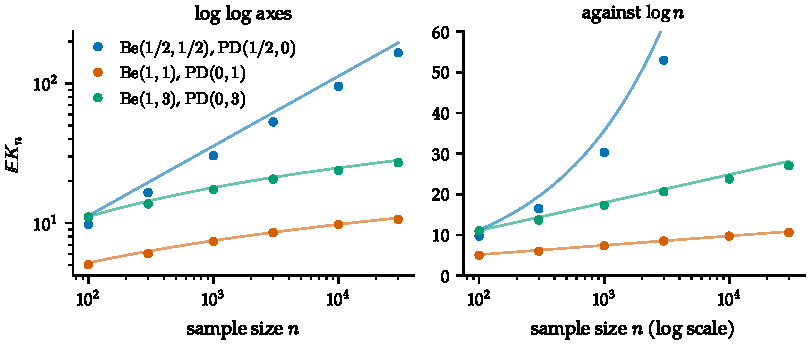
\includegraphics{figures/mp_growth.pdf}
\caption{Expected number of occupied blocks under the species sampling prior matched by
Theorem \ref{mp:thm:main} to three shrinkage priors. Left, log log axes, where only $a<1$
produces a straight line; the horseshoe slope of $0.498$ agrees with the predicted
$n^{1/2}$. Right, plotted against $\log n$, where only $a=1$ produces a straight line, with
slopes $1.005$ and $2.835$ against the predicted $\theta=1$ and $3$. Sixty replicates of the
Chinese restaurant process at each of six sample sizes. Dots are the replicate means and curves the exact means from \eqref{mp:eq:EKexact}.}
\label{mp:fig:growth}
\end{figure}

\subsection{Inflation of the additive genetic variance, and its repair}
\label{mp:sec:numB}

We simulate $L=400$ unlinked biallelic loci with frequencies uniform on $[0.1,0.9]$,
genotypes in Hardy Weinberg proportions, five per cent of loci causal with standard normal
effects, a pairwise epistatic contribution among the causal loci, and independent
environmental noise. This is deliberately favourable to the additive model: the loci are
independent, so $N^{-1}X^\top X$ is $I_p$ up to sampling fluctuations of order $N^{-1/2}$ and
linkage disequilibrium plays no part. Because $p=400$ is at least $N$ at the two smallest sample
sizes, the least squares projection itself is not available there (Corollary
\ref{mp:cor:saturate}), and we use instead its orthogonal design form, the marginal
coefficients $\hat\beta=X^\top y/N$ and $\hat\sigma_A^2=\|\hat\beta\|^2$, which coincide with
the projection when $X^\top X=NI$. This is a linear smoother and Proposition
\ref{mp:prop:optimismgen} applies to it, with one difference worth noting: each marginal
coefficient absorbs the effects of the other loci as noise, so its noise variance is about
$(\sigma_A^2+\sigma^2)/N$ rather than $\sigma^2/N$. The predicted ratio of fitted to true
additive variance is therefore $1+p(\sigma_A^2+\sigma^2)/(N\sigma_A^2)$. With the simulated
averages $\sigma_A^2\approx20$ and $\sigma^2\approx1.9$ this is $3.18$, $2.10$, $1.55$,
$1.27$ and $1.14$ at the five sample sizes. We compare this estimator with the horseshoe
posterior mean, computed by one dimensional quadrature in $\kappa$.

\begin{table}[t]
\centering
\begin{adjustbox}{max width=\textwidth}
\begin{tabular}{lrrrrr}
\toprule
$N$ & 200 & 400 & 800 & 1600 & 3200 \\
\midrule
unregularised projection, orthogonal design form & 3.09 & 2.09 & 1.55 & 1.27 & 1.14 \\
species sampling prior, $\tau=L^{-1/2}$ & 0.65 & 0.81 & 0.89 & 0.94 & 0.98 \\
species sampling prior, oracle $\tau$ & 0.80 & 0.89 & 0.93 & 0.96 & 0.98 \\
\bottomrule
\end{tabular}
\end{adjustbox}
\caption{Estimated $\sigma_A^2$ divided by the true $\sigma_A^2$, $L=400$ loci, 40
replicates. The first row is the orthogonal design form of Fisher's projection \eqref{mp:eq:ewens10} fitted from data, the marginal coefficients $\hat\beta=X^\top y/N$, which coincide with the projection when $X^\top X=NI$. Values
above one indicate inflation. The second row uses the global scale $\tau=L^{-1/2}$ that
Theorem \ref{mp:thm:effsize} identifies as canonical, in units of the coefficient standard
error, which is estimated by the median absolute deviation of the coefficients; nothing
about the truth is used. The third row uses the oracle scale $\sqrt{q/L}$ with $q$ the true
number of causal loci. Monte Carlo standard errors of the first row are $0.053$ at $N=200$
falling to $0.008$ at $N=3200$.}
\label{mp:tab:sigmaA}
\end{table}

At $N=200$, that is at half the number of loci, the fitted projection, in its orthogonal design form, reports an additive
genetic variance three times the truth. The observed ratios $3.09$, $2.09$, $1.55$, $1.27$
and $1.14$ track the predicted $3.18$, $2.10$, $1.55$, $1.27$ and $1.14$, the largest
discrepancy being under two Monte Carlo standard errors, and the bias is still fourteen per
cent at $N=3200$. The species
sampling prior is conservative, understating $\sigma_A^2$ at small $N$ and approaching the
truth from below, but it never inflates. For heritability estimation, which is the applied
form of this question, the direction of the error matters as much as its size: a procedure
that overstates additive variance overstates the response to selection, and by Example
\ref{mp:ex:over} it may report a substantial additive variance in a population sitting exactly
at an equilibrium where the true value is zero.

The comparison between the second and third rows of Table \ref{mp:tab:sigmaA} is the one we
regard as most informative, and it is a direct test of Theorem \ref{mp:thm:effsize}. The second
row is fully data driven: the global scale is set to $L^{-1/2}$, the value the theorem
identifies as the unique power of $L$ at which the effective model size reproduces the
species sampling discovery rate, and $\sigma$ is estimated from the median absolute deviation
of the fitted coefficients. The third row is given the true number of causal loci. The gap
between them is $0.15$ at $N=200$ and closes to $0.01$ by $N=3200$. The theory driven choice
therefore recovers almost all of what the oracle knows, and the value of Theorem
\ref{mp:thm:effsize} is precisely that it removes the need for the oracle.

It is worth recording why the theory driven scale performs so well here, since the reason is
partly an accident of the design. At $\tau=L^{-1/2}$ the prior effective model size
\eqref{mp:eq:effsize} is $L\,\E(1-\kappa)=L\tau/(1+\tau)=19.05$, and Corollary
\ref{mp:cor:growth} gives the leading term $L^{1-a}=L^{1/2}=20$. The simulation has twenty
causal loci, because five per cent of four hundred is twenty and $\sqrt{400}$ is also twenty.
The prior is therefore expecting almost exactly the right number of signals, which is
flattering. What is not an accident is that the prior arrives at that expectation without
being told, and that Corollary \ref{mp:cor:growth} is what tells one what to expect at other
values of $L$.

\begin{figure}[t]
\centering
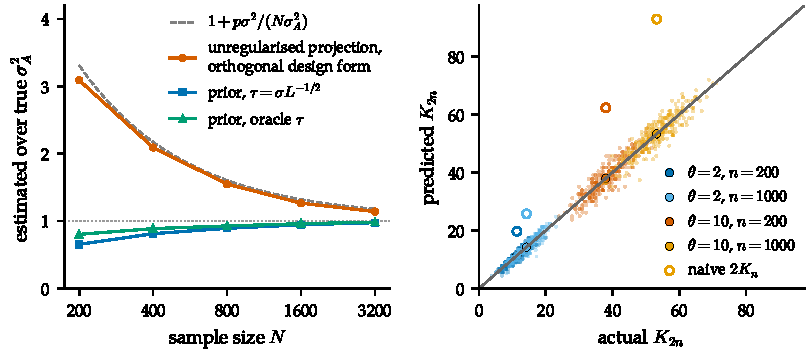
\includegraphics{figures/mp_p1.pdf}
\caption{Left, estimated over true additive genetic variance against sample size with
$L=400$ loci; the unregularised projection, in its orthogonal design form, is inflated by $p\sigma^2/(N\sigma_A^2)$, where here $\sigma^2$
is the noise variance of a coefficient times $N$ (the dashed reference curve), while the
species sampling prior never inflates. In the legend $\sigma L^{-1/2}$ denotes the canonical
global scale $L^{-1/2}$ in units of the estimated coefficient standard error. Right,
predicting the number of distinct alleles in $2n$ genes from a sample of $n$ using the Ewens
Sampling Formula, 300 replicates in each of four settings, against the naive prediction
$2K_n$.}
\label{mp:fig:p1}
\end{figure}

\subsection{Rare variant discovery}
\label{mp:sec:numC}

The right panel of Figure \ref{mp:fig:p1} addresses a question of current applied interest: how
many new variants appear if the sample is doubled? Estimating $\theta$ from $K_n$ by
Propositions \ref{mp:prop:suff} and \ref{mp:prop:feller} and predicting $\E K_{2n}$ gives, over
300 replicates:

\begin{center}
\begin{adjustbox}{max width=\textwidth}
\begin{tabular}{lrrrr}
\toprule
& $\theta=2,\ n=200$ & $\theta=2,\ n=1000$ & $\theta=10,\ n=200$ & $\theta=10,\ n=1000$ \\
\midrule
$K_n$ observed      & 9.84  & 12.87 & 31.14 & 46.42 \\
predicted $K_{2n}$  & 11.25 & 14.25 & 37.96 & 53.28 \\
actual $K_{2n}$     & 11.34 & 14.22 & 37.97 & 53.23 \\
mean relative error & 9.3\% & 7.3\% & 6.0\% & 4.3\% \\
naive $2K_n$ over actual $K_{2n}$ & 1.74 & 1.81 & 1.64 & 1.74 \\
\bottomrule
\end{tabular}
\end{adjustbox}
\end{center}

The prediction is essentially unbiased. This is the species sampling prior doing what a
sparsity prior is asked to do, namely to say how many discoveries to expect, and doing it
from the model rather than from a tuning constant. The relevant comparison is not against a
competitor procedure but against the naive answer, which is that doubling the sample doubles
the discoveries; the table shows the true increase is between ten and twenty two per
cent across the four settings, so the naive prediction $2K_n$ overstates $K_{2n}$ by a factor
of between $1.6$ and $1.8$.

The structure of the calculation is worth making explicit, because it is the same in every
application of the frequency spectrum. One observes $K_n$, inverts $\E K_n(\theta)=K_n$ using
Proposition \ref{mp:prop:feller} to obtain $\hat\theta$, and evaluates $\E K_{2n}(\hat\theta)$.
No new data enters; the extrapolation is carried entirely by the functional form of
$\E K_n(\theta)$, which is $\sum_{j=0}^{n-1}\theta/(\theta+j)$ at $\alpha=0$. The accuracy in
the table therefore measures whether that functional form is right, and the errors of four to
nine per cent are consistent with the sampling variability of $\hat\theta$ implied by
Proposition \ref{mp:prop:feller} rather than with any bias in the extrapolation itself.

Two cautions. The relative error improves with $n$ and with $\theta$, as it should, since
both increase $K_n$ and hence the information about $\theta$; a study with few observed
alleles will predict badly, and the interval of Section \ref{mp:sec:numD} is the right way to
report that. And doubling is a short extrapolation. Predicting $K_{10n}$ from $K_n$ rests
much more heavily on the assumed value of $\alpha$, since by \eqref{mp:eq:Kn} the two candidate
growth laws diverge, and there Corollary \ref{mp:cor:singleton} rather than $K_n$ alone should
be doing the work.

\subsection{Sensitivity to the assumed sparsity level}
\label{mp:sec:sens}

Corollary \ref{mp:cor:growth} is a statement about what a prior will do, not about what is true,
so it is worth asking what happens when the assumed $\alpha$ is wrong. The two failure modes
are asymmetric and it is useful to say why.

Suppose the truth has $q_n$ contributing variants in dimension $n$ and the analyst uses a
prior with parameter $a$, hence assumed rate $n^{1-a}$. If $q_n\gg n^{1-a}$, the prior is too
conservative: by \eqref{mp:eq:aj} the expected number of occupied blocks is a hard ceiling in
expectation, and the excess signals are shrunk toward zero regardless of their magnitude.
This is the lasso failure in the ultra sparse regime, and no adjustment of the global scale
repairs it, because the global scale moves $\theta$ and by \eqref{mp:eq:Kn} at $\alpha=0$ the
rate is $\theta\log n$, which is logarithmic for every $\theta$. Multiplying $\theta$ by ten
buys a factor of ten, not a change of rate.

If instead $q_n\ll n^{1-a}$, the prior is too liberal, and the consequence is overdiscovery
at a rate the multiplicity structure does not control. This failure is visible: it shows up
as a fitted spectrum with too many singletons relative to the observed one, and by Corollary
\ref{mp:cor:singleton} the discrepancy is measurable. The asymmetry is therefore practical as
well as formal. Assuming too little sparsity produces an error one can detect from the data;
assuming too much produces an error one cannot, because the missing signals never appear in
any output. When in doubt the argument favours the smaller $a$.

\subsection{Uncertainty in the mutation parameter}
\label{mp:sec:numD}

Using \eqref{mp:eq:poch} and the exact posterior, at $n=100$ and $\theta=5$ the median $95\%$
credible interval over 400 replicates is $[2.53,8.52]$, a width of $5.99$, that is $120\%$ of
$\theta$. Its frequentist coverage, computed exactly by summing over the law of $K_n$ given by
Proposition \ref{mp:prop:feller}, is $0.943$; the empirical coverage in the 400 replicates was
$0.915$, which is $2.4$ Monte Carlo standard errors below that. At $n=1000$ the width is still $83\%$ of
$\theta$, with exact coverage $0.938$, and at $\theta=1$, $n=100$ it is twice $\theta$. The slow improvement reflects
the $(\log n)^{-1/2}$ rate implied by Proposition \ref{mp:prop:feller}. Figure \ref{mp:fig:theta}
displays a representative posterior against the customary point estimate.

\begin{figure}[t]
\centering
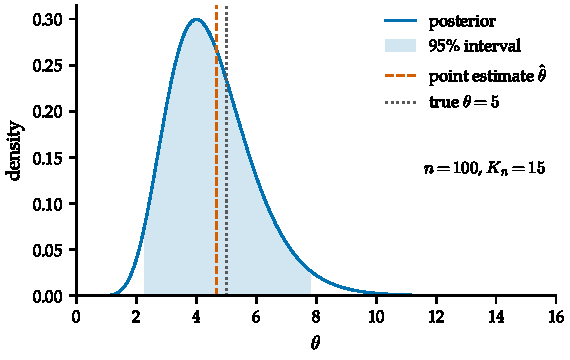
\includegraphics{figures/mp_theta.pdf}
\caption{Exact posterior for $\theta$ under the Pochhammer prior \eqref{mp:eq:poch} for a
representative sample with $n=100$ and $K_n=15$ drawn at $\theta=5$, against the point
estimate $\hat\theta=4.66$ solving $\E K_n(\theta)=K_n$. The posterior mean is $4.53$ and the
$95\%$ interval $[2.25,7.83]$. The point estimate is accurate on average and conceals
uncertainty of order $\theta$ itself.}
\label{mp:fig:theta}
\end{figure}

Since by Corollary \ref{mp:cor:cases} $\theta$ fixes the implied sparsity level, uncertainty of
this magnitude propagates directly into any downstream discovery statement, and reporting a
single value of $\theta$ understates it.

The slowness is structural rather than a defect of the estimator. By Proposition
\ref{mp:prop:feller}, $K_n$ is a sum of independent indicators with
$\E K_n\sim\theta\log n$ and $\Var K_n\sim\theta\log n$, so the Fisher information about
$\theta$ accumulates like $\log n$ and the standard error of any estimator falls like
$(\log n)^{-1/2}$. Going from $n=100$ to $n=1000$ multiplies the information at $\theta=5$ by about
$2.1$, not by ten (the leading order ratio is $3/2$). This is a feature of the infinite alleles model and not of the Bayesian
treatment: the point estimate is exactly as uncertain, and merely does not say so.

There is a practical consequence for the design of studies. If the object of interest is
$\theta$ itself, or a discovery count derived from it, then increasing the sample size is an
inefficient way to buy precision, and pooling independent loci that share a common $\theta$
is far better, since by Proposition \ref{mp:prop:aug} the information from $m$ loci adds. The
augmented scheme of Section \ref{mp:sec:conj} is written for exactly that case.

\subsection{Simulation design}
\label{mp:sec:design}

For reproducibility we record the design of the four studies above. Discovery rates: the
two parameter Chinese restaurant process is run to $n=3\times10^4$ with 60 independent
replicates per parameter setting, and $\E K_n$ is recorded at six checkpoints; the log log
slope is fitted by least squares across those checkpoints. Additive genetic variance:
$L=400$ loci, allele frequencies uniform on $[0.1,0.9]$, genotypes drawn as
$\mathrm{Bin}(2,p_\ell)$ and standardised, twenty causal loci with standard normal effects,
an epistatic term formed from ten products of disjoint pairs of causal loci scaled by $0.3$,
environmental noise standard normal, 40 replicates at each of five sample sizes. The
horseshoe posterior mean of each coefficient is computed by a $400$ point midpoint rule in
$\kappa$ on $(0,1)$ in the normal means model $\hat\beta_j\sim N(\beta_j,s^2)$, with $s$
estimated by the median absolute deviation of the fitted coefficients, and with the global
scale set either to the canonical value $L^{-1/2}$ or to the oracle value $\sqrt{q/L}$ where
$q$ is the number of causal loci; the gap between the two rows of Table \ref{mp:tab:sigmaA}
is exactly what knowing $q$ is worth. Rare variant discovery: partitions generated by the Feller coupling of
Proposition \ref{mp:prop:feller}, subsampled to size $n$ from a realisation of size $2n$, 300
replicates. Mutation parameter: 400 replicates, posterior computed on a $4000$ point
geometric grid in $\theta$ on $[10^{-2},400]$ with the prior \eqref{mp:eq:poch}.

Two caveats about what these studies do and do not establish. They are illustrations of the
theory, not comparisons against competing methods, and in particular we make no claim about
the relative performance of the horseshoe against genomic prediction methods designed for
this problem. And the additive genetic variance study uses a nearly orthogonal design, so
by Proposition \ref{mp:prop:gram} it isolates the sampling contribution to the inflation and
excludes the linkage disequilibrium contribution of Example \ref{mp:ex:twolocus}, which is
present in real data and is additional.

\subsection{What the four studies show, taken together}
\label{mp:sec:together}

The four studies are not four unrelated demonstrations. Read in order they trace one
argument.

Section \ref{mp:sec:numA} establishes that the dictionary of Theorem \ref{mp:thm:main} has
operational content, in that the partition matched to a prior labelled by $(a,b)$ produces the discovery rate
$n^{1-a}$ that Corollary \ref{mp:cor:growth} predicts, to within the half per cent that the
fitted slope $0.498$ against $0.5$ represents. Without this the dictionary would be a
curiosity.

Section \ref{mp:sec:numB} establishes that the problem the dictionary is meant to solve is
real, and quantifies it in Fisher's own estimand. The threefold inflation at $N=200$ is not
an artefact of a badly chosen design; the design is nearly orthogonal and the loci are
independent.
By Proposition \ref{mp:prop:gram} realistic linkage disequilibrium adds a further, separately
signed error to the estimand itself.

Section \ref{mp:sec:numC} shows that when the species sampling prior is used for the thing it
is naturally suited to, namely predicting how many further variants a larger sample will
reveal, it is accurate to within about nine per cent, against a naive doubling rule which overstates
the count by a factor of between $1.6$ and $1.8$. This is the positive case for the
machinery, as against the negative case made by Section \ref{mp:sec:numB}.

Section \ref{mp:sec:numD} then closes the loop by showing what is not known. If the prior is
indexed by $\theta$ and $\theta$ is uncertain by an amount comparable to itself, then the
implied discovery count inherits that uncertainty, and the customary practice of reporting a
point estimate suppresses it. Combined with Section \ref{mp:sec:timescale}, which shows that
$\theta$ is in addition convention dependent, the practical recommendation is to report the
pair $(\alpha,\theta)$ with $\alpha$ as the invariant of scientific interest and $\theta$
with a posterior attached.

\section{Genetic implications}
\label{mp:sec:genetics}

\paragraph{Heritability.} Corollary \ref{mp:prop:optimism} and Table \ref{mp:tab:sigmaA} identify
an upward bias in additive genetic variance proportional to the number of fitted average
effects. Any procedure that estimates $\sigma_A^2$ by fitting an additive model across many
loci and reporting the explained sum of squares inherits this bias exactly. The correction is
not a matter of taste in regularisation; it is forced by the dimension of the projection in
Fisher's own definition. Proposition \ref{mp:prop:optimismgen} gives the general form and shows
what any competing estimator must trade.

\paragraph{The frequency spectrum as a prior.} Fisher's log series is usually read
descriptively. Theorem \ref{mp:thm:spectrum} shows it is the shrinkage profile with its size bias removed, so
reading it as a prior is not a metaphor but an identity, and Corollary \ref{mp:cor:cases}
sharpens the point: the uniform shrinkage prior corresponds to the Ewens Sampling Formula at
$\theta=1$, and the Strawderman Berger prior is its $\alpha=1/2$ counterpart
$\PD(1/2,1/2)$. This gives the genetics literature a second use for a quantity it already
computes, and gives the statistics literature a generative account of priors it has been
choosing on grounds of convenience.

\paragraph{Which prior for which regime.} Corollary \ref{mp:cor:growth} gives a design rule. If
the biology says the number of contributing variants grows polynomially in the sample, a
prior with $a<1$ is required and no amount of tuning rescues $a=1$. If the number is
genuinely logarithmic, an $a=1$ prior is appropriate and an $a<1$ prior overdiscovers. The
choice is a genetic statement, not a computational one, and by Corollary \ref{mp:cor:singleton}
it can be checked against the observed singleton count rather than asserted.

\paragraph{Multiple testing.} The multiplicity penalty in a global local analysis is usually
described as arising automatically from the shared global scale. Theorem \ref{mp:thm:spectrum}
says what it is: the expected number of discoveries is $\E K_n=\sum_j\E a_j$ with $\E a_j$
given by \eqref{mp:eq:aj}, so the penalty is a functional of the frequency spectrum. In a
genetic application the multiplicity adjustment can therefore be calibrated against the
observed spectrum.

\paragraph{Effective sizes and effective sparsity.} \citet{mp:ewenshossjer2025} show that the
inbreeding, variance and eigenvalue effective population sizes are distinct quantities which
coincide for monoecious Wright Fisher populations and diverge otherwise, and that which to
use depends on whether one cares about short or long term loss of heterozygosity. The
identity by descent probability $\pi_2$ on which the first of these rests is developed in
detail by \citet{mp:thompson2013}. The
parallel is exact: there is no such thing as \emph{the} sparsity level either. Theorem
\ref{mp:thm:main} says which two parameter family the alternatives inhabit and Corollary
\ref{mp:cor:growth} says what distinguishes them.

\section{Limitations}
\label{mp:sec:limits}

We set out what we take to be the weak points of the argument, in decreasing order of
seriousness.

\paragraph{The partition identity is unproved.} As Remark \ref{mp:rem:open} states, Theorems
\ref{mp:thm:main} and \ref{mp:thm:spectrum} concern the random discrete distribution generated by
a normalised subordinator, while the working object in \eqref{mp:eq:gl} is a set of independent
weights on a fixed index set. The two agree in the marginal law of a size biased pick and in
the mean intensity of the atoms, which is what Theorem \ref{mp:thm:spectrum} establishes, but
we have not shown that the exchangeable partitions agree. What survives without that
identification is the first moment: Theorem \ref{mp:thm:effsize} proves the discovery rate
directly for \eqref{mp:eq:gl}, and Table \ref{mp:tab:tpb} confirms it numerically. Statements
about the whole law of the number of discoveries, by contrast, do not transfer, as
Proposition \ref{mp:prop:fluct} shows.

\paragraph{The global scale is doing work.} The prior \eqref{mp:eq:gl} has two levels, and the
$\Be(a,b)$ description of $\kappa$ holds at a fixed global scale $\tau$. Allowing $\tau$ to
be estimated changes the marginal law of $\kappa$ and therefore, formally, moves the implied
$(\alpha,\theta)$. Our reading is that estimating $\tau$ is how the data speaks about
$\theta$ while $a$ continues to fix $\alpha$, which is consistent with the separation of rate
from level described in Section \ref{mp:sec:timescale}, but we have not proved it.

\paragraph{The additive genetic variance study is idealised.} Section \ref{mp:sec:design}
records that the design is nearly orthogonal, which favours the shrinkage estimator; the
oracle global scale is reported only for comparison and the headline row does not use it.
The orthogonality also suppresses the linkage
disequilibrium contribution of Example \ref{mp:ex:twolocus}, which acts on the estimand rather
than the estimator and which no regularisation addresses. The net effect on a real analysis
is not something we can predict from these simulations.

\paragraph{Epistasis is treated as noise.} Throughout, epistatic contributions are absorbed
into $\eta$ in \eqref{mp:eq:reg} and therefore into $\sigma^2$. This is the same convention
Fisher adopts and that \citet{mp:ewens2024} analyses, and it is what makes $\sigma_A^2$ a
projection rather than a decomposition. It means, however, that the inflation
$p\sigma^2/N$ grows with the amount of epistasis, so that the very phenomenon which makes
the additive projection an incomplete summary also makes its naive estimate worse.

\paragraph{One parameter, one spectrum.} The Ewens Sampling Formula assumes selective
neutrality and a single time homogeneous mutation rate. Real spectra are shaped by
selection, by demography and by ascertainment. Corollary \ref{mp:cor:singleton} offers a
diagnostic, in that the growth rate of the singleton count identifies $\alpha$, but a
mismatch between the observed and predicted spectrum has many possible causes and the prior
is only one of them.

\section{Discussion}
\label{mp:sec:disc}

The mathematical claims are Theorems \ref{mp:thm:main} and \ref{mp:thm:spectrum}, which place the
shrinkage priors of sparse Bayesian statistics inside the two parameter Poisson Dirichlet
family and identify the frequency spectrum with the shrinkage density once its size bias is removed. The
practical claim is Corollary \ref{mp:cor:growth}, which converts the identification into a
statement about how many signals a given prior will ever find. The genetic claim is
Corollary \ref{mp:prop:optimism}, that Fisher's additive genetic variance, estimated by fitting
his own definition, is inflated by an amount proportional to the ratio of parameter count to sample size.

Four problems remain open. The first is the partition level identification of Remark
\ref{mp:rem:open}. The second is whether the $n^{1/2}$ rate for the horseshoe coincides with
the sparsity regime in which its posterior is known to contract at the minimax rate; if so,
the optimal global scale is a statement about $\theta$. The third is the behaviour of
Proposition \ref{mp:prop:optimismgen} under realistic linkage disequilibrium, where
$\mathrm{tr}(H^\top H)$ must be computed from an empirical Gram matrix with strong local
correlation, and where the effective number of independent parameters is smaller than $p$.
The fourth is inference for $\alpha$ itself. Corollary \ref{mp:cor:singleton} suggests that the
singleton count identifies $\alpha$, which would make the sparsity level estimable from the
frequency spectrum rather than chosen, and would close the circle by letting the genetics
determine the prior.



\section{Proofs}
\label{mp:app:proofs}

\begin{proof}[Proof of Proposition \ref{mp:prop:onelocus}]
Write $Q(\beta)=\sum_u\sum_v p_up_v(m_{uv}-\beta_u-\beta_v)^2$. Each $\beta_u$ occurs in the
terms with first index $u$ and in those with second index $u$, and by symmetry of $m$ and of
$P$ these contribute equally, so
$\partial Q/\partial\beta_u=-4\sum_v p_up_v(m_{uv}-\beta_u-\beta_v)$. Setting this to zero
and dividing by $4p_u>0$ gives $m_{u\cdot}-\beta_u-\bar\beta=0$ with
$\bar\beta=\sum_vp_v\beta_v$, that is $\beta_u=m_{u\cdot}-\bar\beta$. Multiplying by $p_u$
and summing gives $\bar\beta=\bar m-\bar\beta$, so $\bar\beta=\bar m/2$ and
$\beta_u=m_{u\cdot}-\bar m/2$. Then $\bar m=2\bar\beta=2\sum_up_u\beta_u$ and
$\beta_u-\bar\beta=m_{u\cdot}-\bar m=a_u$. The fitted value for genotype $(u,v)$ is
$\beta_u+\beta_v$, with mean $2\bar\beta=\bar m$, so the variance removed is
$\sum_u\sum_vp_up_v(\beta_u+\beta_v-\bar m)^2=\sum_u\sum_vp_up_v(a_u+a_v)^2=2\sum_up_ua_u^2$,
the cross term vanishing because $\sum_up_ua_u=\bar m-\bar m=0$.
\end{proof}

\begin{proof}[Proof of Proposition \ref{mp:prop:wlsconsistency}]
We assume that the genotype set is finite, that the $\varepsilon_i$ are independent of the
$g_i$ and of each other and are identically distributed with mean zero and variance $\sigma^2$, and that redundant gene
content functions have been removed (for instance one allele per locus, since allele counts at
a locus sum to two), so that the population Gram matrix
$A=\sum_gP_g\,\mathbf a_g\mathbf a_g^\top=\mathcal A^\top W\mathcal A$ is nonsingular. Here
$\mathbf a_g$ is the vector of gene contents of genotype $g$, so that
$\sum_{(g)}\beta_{ij}=\mathbf a_g^\top\beta$. Expanding the square,
\[
\frac1N\sum_{i=1}^N\big(y_i-\mathbf a_{g_i}^\top\beta\big)^2
=\sum_g\hat P_g\big(m_g-\mathbf a_g^\top\beta\big)^2
+\frac2N\sum_{i=1}^N\varepsilon_i\big(m_{g_i}-\mathbf a_{g_i}^\top\beta\big)
+\frac1N\sum_{i=1}^N\varepsilon_i^2 ,
\]
with $\hat P_g=N^{-1}\#\{i:g_i=g\}$. The first term is \eqref{mp:eq:ewens10} at $\hat P_N$. The
whole expression is a quadratic $\beta^\top A_N\beta-2\beta^\top b_N+c_N$ whose coefficients are
finitely many sample averages; by the strong law $A_N\to A$, $b_N\to b=\sum_gP_g\mathbf a_gm_g$
and $c_N\to c=\sum_gP_gm_g^2+\sigma^2$ almost surely, the cross terms involving $\varepsilon_i$
having mean zero. The difference between the criterion and $Q(\beta)+\sigma^2$ is bounded by
$\|A_N-A\|\,\|\beta\|^2+2\|b_N-b\|\,\|\beta\|+|c_N-c|$, which tends to zero uniformly on
compacta. Finally $A_N$ is nonsingular for all large $N$, and the minimiser
$A_N^{-1}b_N$ converges to $A^{-1}b$, which is the minimiser of $Q$, that is Fisher's vector
of average effects.
\end{proof}

\begin{proof}[Proof of Proposition \ref{mp:prop:optimismgen}]
$\E\|Hy\|^2=\|HX\beta\|^2+\E\|H\eta\|^2=\|HX\beta\|^2+\sigma^2\mathrm{tr}(H^\top H)$, using
$\E\eta=0$ and $\Var\eta=\sigma^2I$. Divide by $N$.
\end{proof}

\begin{proof}[Proof of Proposition \ref{mp:prop:hoppe}]
Fix a partition of $\{1,\dots,n\}$ into blocks $B_1,\dots,B_k$ of sizes $n_1,\dots,n_k$, listed
in order of their least elements. The urn produces this partition exactly when draw $j$ is
black whenever $j$ is the least element of its block, and otherwise draws the colour of the
block containing $j$; the names of the colours do not matter. Before draw $j$ the total mass
is $\theta+j-1$. If $j$ is the least element of a block the required probability is
$\theta/(\theta+j-1)$; if $j$ is the $r$th smallest element of $B_i$, $r\ge2$, the colour of
$B_i$ then has mass $r-1$ and the required probability is $(r-1)/(\theta+j-1)$. Multiplying
over $j$, the denominators give $\prod_{j=1}^n(\theta+j-1)=\theta_{(n)}$, and the numerators
give $\theta$ once per block and $1\cdot2\cdots(n_i-1)$ within block $i$, that is
$\theta^k\prod_i(n_i-1)!$. This is \eqref{mp:eq:eppf}.
\end{proof}

\begin{proof}[Proof that the map of Theorem \ref{mp:thm:main} is onto]
Let $a\in(0,1]$, $b>0$ and set $\alpha=1-a\in[0,1)$, $\theta=a+b-1$. The $\GEM$ constraint
$\theta>-\alpha$ reads $a+b-1>a-1$, that is $b>0$, which holds. Conversely for
$\alpha\in[0,1)$ and $\theta>-\alpha$ set $a=1-\alpha\in(0,1]$ and $b=\theta+\alpha>0$. The
two maps are mutual inverses.
\end{proof}

\begin{proof}[Proof of Theorem \ref{mp:thm:spectrum}]
By definition a size biased pick satisfies
$\Prob(W\in A)=\E\sum_iP_i\mathbf 1(P_i\in A)$. Taking $h(x)=x\mathbf 1(x\in A)$, which is
bounded and vanishes at the origin, in the definition of $\nu$ gives
$\Prob(W\in A)=\int_Ax\nu(x)\dd x$ for every Borel $A\subset(0,1)$, so $f_W(x)=x\nu(x)$.
For \eqref{mp:eq:aj}, condition on $(P_i)$. Given the frequencies, the number of the $n$
independent draws that land on atom $i$ is $\mathrm{Bin}(n,P_i)$, so the number of atoms
represented exactly $j\ge1$ times is $\sum_i\mathbf 1\{\mathrm{Bin}(n,P_i)=j\}$, with
conditional expectation $\sum_i h_j(P_i)$ where $h_j(x)=\binom{n}{j}x^j(1-x)^{n-j}$. This $h_j$
is bounded and vanishes at the origin because $j\ge1$, so taking expectations gives
$\E a_j=\binom{n}{j}\int_0^1x^j(1-x)^{n-j}\nu(x)\dd x$. Substituting $\nu=x^{-1}f_\kappa$
gives the display.
\end{proof}

\begin{proof}[Proof of Theorem \ref{mp:thm:effsize}]
Write $Z=\kappa_1/(1-\kappa_1)$. If $\kappa_1\sim\Be(a,b)$ then $Z$ has the beta prime law
with density $f(z)=z^{a-1}(1+z)^{-a-b}/B(a,b)$ on $(0,\infty)$. Since
$\kappa_\tau/(1-\kappa_\tau)=\tau^{-2}Z$ by the definition of $\kappa_\tau$, we have
$1-\kappa_\tau=\tau^2/(\tau^2+Z)$ and therefore
\[
\E(1-\kappa_\tau)=\int_0^\infty \frac{\tau^2}{\tau^2+z}\,f(z)\dd z .
\]
Substitute $z=\tau^2 w$, so that $\dd z=\tau^2\dd w$ and
\[
\E(1-\kappa_\tau)=\tau^{2}\int_0^\infty\frac{f(\tau^2w)}{1+w}\dd w
=\frac{\tau^{2a}}{B(a,b)}\int_0^\infty\frac{w^{a-1}(1+\tau^2w)^{-a-b}}{1+w}\dd w .
\]
For $0<a<1$ the integrand is dominated by $w^{a-1}/(1+w)$, which is integrable at both ends,
so dominated convergence gives
$\int_0^\infty w^{a-1}(1+w)^{-1}\dd w = \pi/\sin(\pi a)$ in the limit, which is the first
display. For $a=1$ the limiting integrand $(1+w)^{-1}$ is not integrable at infinity, and the cutoff
is exhibited by the further substitution $w=v/\tau^2$, under which
\[
\int_0^\infty\frac{(1+\tau^2w)^{-1-b}}{1+w}\dd w
=\int_0^\infty\frac{(1+v)^{-1-b}}{\tau^2+v}\dd v
=2\log(1/\tau)+O(1).
\]
To see the last step, split the range at $v=1$. On $(0,1)$ write
$(1+v)^{-1-b}=1+\{(1+v)^{-1-b}-1\}$: the first part integrates to
$\log\{(1+\tau^2)/\tau^2\}=2\log(1/\tau)+o(1)$, and the second has absolute value at most
$(1+b)v/(\tau^2+v)\le1+b$, so contributes $O(1)$. On $(1,\infty)$ the integrand is at most
$(1+v)^{-1-b}$, which is integrable, so that part is $O(1)$ too. With $B(1,b)=1/b$ this is the
second display. Setting $p=n$ and $\tau_n=n^{-1/2}$ gives $\tau_n^{2a}=n^{-a}$, hence
$\E m_n = n\,\E(1-\kappa_{\tau_n})\sim C\,n^{1-a}$ for $a<1$, and for $a=1$,
$\E m_n = n\cdot 2b\,n^{-1}\cdot\tfrac12\log n = b\log n$.
\end{proof}

\begin{proof}[Proof of Lemma \ref{mp:lem:second}]
As in the previous proof, $1-\kappa_\tau=\tau^2/(\tau^2+Z)$ with $Z$ beta prime, so
\[
\E(1-\kappa_\tau)^2=\int_0^\infty\Big(\frac{\tau^2}{\tau^2+z}\Big)^2 f(z)\dd z
=\frac{\tau^{2a}}{B(a,b)}\int_0^\infty\frac{w^{a-1}(1+\tau^2w)^{-a-b}}{(1+w)^{2}}\dd w
\]
after $z=\tau^2w$. For $0<a<1$ the integrand is dominated by $w^{a-1}(1+w)^{-2}$, which is
integrable, and dominated convergence gives
$\int_0^\infty w^{a-1}(1+w)^{-2}\dd w=B(a,2-a)$.
\end{proof}

\begin{proof}[Proof of Corollary \ref{mp:cor:agree}]
Under Theorem \ref{mp:thm:main} the matched parameters are $\alpha=1-a$ and $\theta=a+b-1$, so
$n^{\alpha}=n^{1-a}$, which is the exponent in Theorem \ref{mp:thm:effsize}, and at $a=1$ the
species sampling rate is $\theta\log n=b\log n$, which is the second display. For the
constants, \eqref{mp:eq:Kn} gives
$\Gamma(\theta+1)/\{\alpha\Gamma(\theta+\alpha)\}=\Gamma(a+b)/\{(1-a)\Gamma(b)\}$, while
Theorem \ref{mp:thm:effsize} gives $\pi/\{B(a,b)\sin(\pi a)\}$. Using
$\Gamma(a)\Gamma(1-a)=\pi/\sin(\pi a)$ and $B(a,b)=\Gamma(a)\Gamma(b)/\Gamma(a+b)$, the
latter equals $\Gamma(1-a)\Gamma(a+b)/\Gamma(b)$. The ratio of the two constants is therefore
$(1-a)\Gamma(1-a)=\Gamma(2-a)$, which on $a\in(0,1]$ attains its minimum
$\Gamma(1.4616)\approx0.8856$ and its maximum $\Gamma(1)=1$ at $a=1$.
\end{proof}

\begin{proof}[Proof of Corollary \ref{mp:cor:logseries}]
With $f_\kappa(x)=\theta(1-x)^{\theta-1}$, \eqref{mp:eq:aj} gives
$\E a_j=\binom{n}{j}\theta B(j,n-j+\theta)
=\frac{n!}{j!(n-j)!}\theta\frac{\Gamma(j)\Gamma(n-j+\theta)}{\Gamma(n+\theta)}
=\frac{\theta}{j}\frac{n!}{(n-j)!}\frac{\Gamma(\theta+n-j)}{\Gamma(\theta+n)}$.
As $n\to\infty$ with $j$ fixed, $n!/(n-j)!\sim n^j$ and
$\Gamma(\theta+n-j)/\Gamma(\theta+n)\sim n^{-j}$, giving $\theta/j$.
\end{proof}

\begin{proof}[Proof of Corollary \ref{mp:cor:singleton}]
With $f_\kappa(x)=\{\pi\sqrt{x(1-x)}\}^{-1}$ and $j=1$, \eqref{mp:eq:aj} gives
$\E a_1=n\pi^{-1}\int_0^1x^{-1/2}(1-x)^{n-3/2}\dd x=n\pi^{-1}B(1/2,n-1/2)$, and
$B(1/2,n-1/2)=\Gamma(1/2)\Gamma(n-1/2)/\Gamma(n)\sim\sqrt\pi\,n^{-1/2}$.
\end{proof}

\begin{proof}[Proof of Proposition \ref{mp:prop:gram}]
The additive projection of $m$ on $z=(z_1,\dots,z_L)$ has coefficient vector $R^{-1}c$ and
explained variance $c^\top R^{-1}c$. Fitting locus $\ell$ alone gives coefficient $c_\ell$
and explained variance $c_\ell^2$. Equality of $c^\top R^{-1}c$ and $c^\top c$ for all $c$
forces $R^{-1}=I$.
\end{proof}

\begin{proof}[Proof of Proposition \ref{mp:prop:pk}]
Let $\mathcal N=\sum_i\delta_{J_i}$ be the Poisson process, so that $T=T(\mathcal N)=\sum_iJ_i$.
Given the frequencies $P_i=J_i/T$, the $n$ draws are independent, and the probability that
they realise a given partition with blocks of sizes $n_1,\dots,n_k$ is
$\sum^{\ne}\prod_{l=1}^kP_{i_l}^{n_l}$, the sum running over ordered $k$ tuples of distinct
atoms $(i_1,\dots,i_k)$. Hence
\[
p(n_1,\dots,n_k)=\E\Big[T^{-n}\sum^{\ne}\prod_{l=1}^kJ_{i_l}^{n_l}\Big].
\]
The awkward factor $T^{-n}$ is removed by the gamma integral
$T^{-n}=\Gamma(n)^{-1}\int_0^\infty t^{n-1}e^{-tT}\dd t$, and since every term is
nonnegative Tonelli's theorem allows the expectation to be taken inside the $t$ integral.
It remains to show that, for each $t>0$,
\[
\E\Big[e^{-tT}\sum^{\ne}\prod_{l=1}^kJ_{i_l}^{n_l}\Big]
=e^{-\psi(t)}\prod_{l=1}^k\xi(n_l,t).
\]
This is the multivariate Mecke equation \citep[Theorem 4.4]{mp:last2017}: for a Poisson
process with intensity $\rho$ and nonnegative $F$,
$\E\sum^{\ne}F(J_{i_1},\dots,J_{i_k};\mathcal N)
=\int\!\cdots\!\int\E F(x_1,\dots,x_k;\mathcal N+\delta_{x_1}+\dots+\delta_{x_k})
\prod_l\rho(x_l)\dd x_l$. Apply it with
$F(x_1,\dots,x_k;\mathcal N)=\prod_lx_l^{n_l}e^{-tT(\mathcal N)}$. Adding the $k$ points
$x_l$ adds $\sum_lx_l$ to $T$, so the integrand factorises as
$\E e^{-tT(\mathcal N)}\prod_lx_l^{n_l}e^{-tx_l}\rho(x_l)$; the integrals over the $x_l$ give
$\prod_l\xi(n_l,t)$, and $\E e^{-tT}=e^{-\psi(t)}$ is Campbell's formula for the Laplace
functional of a Poisson process. Substituting into the $t$ integral gives
\eqref{mp:eq:pkformula}.
\end{proof}

\begin{proof}[Proof of Corollary \ref{mp:cor:growth} and of \eqref{mp:eq:EKexact}]
We first prove the exact formula \eqref{mp:eq:EKexact}. Dividing \eqref{mp:eq:pyeppf} for the
partition with an added singleton block by \eqref{mp:eq:pyeppf} itself, the product in the
numerator gains the factor $\theta+k\alpha$, the denominator gains $\theta+n$, and the new
block contributes $(1-\alpha)_{(0)}=1$. So, given $K_n=k$, draw $n+1$ starts a new block with
probability $(\theta+k\alpha)/(\theta+n)$, and taking expectations, $u_n=\E K_n$ satisfies
\[
u_{n+1}=u_n+\frac{\theta+\alpha u_n}{\theta+n},\qquad n\ge1,\qquad u_1=1 .
\]
For $\alpha=0$ this gives $u_n=1+\sum_{j=1}^{n-1}\theta/(\theta+j)=\sum_{j=0}^{n-1}\theta/(\theta+j)$,
in agreement with Proposition \ref{mp:prop:feller}. For $\alpha>0$ put $v_n=u_n+\theta/\alpha$.
Then $v_{n+1}=v_n(\theta+\alpha+n)/(\theta+n)$ and $v_1=(\theta+\alpha)/\alpha$, so
\[
\begin{aligned}
v_n&=\frac{\theta+\alpha}{\alpha}\prod_{j=1}^{n-1}\frac{\theta+\alpha+j}{\theta+j}
=\frac{\theta+\alpha}{\alpha}\cdot\frac{\Gamma(\theta+\alpha+n)\,\Gamma(\theta+1)}
{\Gamma(\theta+\alpha+1)\,\Gamma(\theta+n)}\\
&=\frac{\Gamma(\theta+1)}{\alpha\,\Gamma(\theta+\alpha)}\cdot
\frac{\Gamma(\theta+\alpha+n)}{\Gamma(\theta+n)},
\end{aligned}
\]
which is \eqref{mp:eq:EKexact}. Since $\Gamma(x+\alpha)/\Gamma(x)\sim x^\alpha$ as
$x\to\infty$, $u_n\sim\Gamma(\theta+1)n^\alpha/\{\alpha\Gamma(\theta+\alpha)\}$, while for
$\alpha=0$ the sum is $\theta\log n+O(1)$; this proves \eqref{mp:eq:Kn}. The corollary follows
on substituting the matched parameters $(\alpha,\theta)=(1-a,a+b-1)$ of Theorem
\ref{mp:thm:main}: the rate is $n^{1-a}$ for $a<1$ and $b\log n$ for $a=1$.
\end{proof}

\begin{proof}[Proof of Lemma \ref{mp:lem:beta}]
$\int_0^1t^{\theta-1}(1-t)^{n-1}\dd t=B(\theta,n)=\Gamma(\theta)\Gamma(n)/\Gamma(\theta+n)$.
\end{proof}

\begin{proof}[Proof of Proposition \ref{mp:prop:aug}]
By \eqref{mp:eq:eppf} and Lemma \ref{mp:lem:beta} the contribution of locus $r$ is
$\theta^{k_r}\Gamma(n_r)^{-1}\int_0^1t_r^{\theta-1}(1-t_r)^{n_r-1}\dd t_r$. Introducing
$t_r$ as latent, the joint density of $(\theta,t_{1:m})$ given the data is proportional to
$p(\theta)\theta^{\sum_rk_r}\prod_rt_r^{\theta-1}(1-t_r)^{n_r-1}$. Reading off the
conditionals gives $t_r\mid\theta\sim\Be(\theta,n_r)$ and
$p(\theta\mid t_{1:m})\propto p(\theta)\theta^{\sum_rk_r}e^{\theta\sum_r\log t_r}$. With
$p(\theta)\propto\theta^{c_0-1}e^{-d_0\theta}$ this is
$\mathrm{Ga}(c_0+\sum_rk_r,\,d_0-\sum_r\log t_r)$, noting $\log t_r<0$ so that the rate is
positive. The Gibbs sampler alternating the two conditionals therefore has the posterior of
$(\theta,t_{1:m})$ as its stationary law, and its $\theta$ marginal is $p(\theta\mid k_{1:m})$
because integrating out $t_{1:m}$ returns the likelihood by Lemma \ref{mp:lem:beta}.
\end{proof}

\section{Notation}
\label{mp:app:notation}

\begin{center}
\begin{adjustbox}{max width=\textwidth}
\begin{tabular}{ll}
\toprule
symbol & meaning \\
\midrule
$n$ & number of genes in a sample \\
$N$ & number of individuals in a regression sample \\
$p,\ L$ & number of fitted average effects, number of loci \\
$K_n$ & number of distinct alleles in a sample of $n$ genes \\
$a_j$ & number of alleles represented exactly $j$ times \\
$\theta$ & mutation parameter, equivalently Pitman's second parameter \\
$\alpha$ & Pitman's first parameter, the discovery exponent \\
$\theta_{(n)}$ & Pochhammer symbol $\Gamma(\theta+n)/\Gamma(\theta)$ \\
$\beta_u,\ a_u$ & average effect and average excess of allele $A_u$ \\
$\sigma_A^2$ & additive genetic variance \\
$\kappa$ & shrinkage weight $1/(1+\tau^2\lambda^2)$ \\
$a,b$ & parameters of the beta law of $\kappa$ \\
$\rho,\ \nu$ & L\'evy density of the subordinator, mean intensity of the atoms \\
$\psi,\ \xi(m,t)$ & Laplace exponent and tilted moments of $\rho$ \\
$H$ & linear smoother, $\hat y=Hy$ \\
$R$ & correlation matrix of standardised coded loci \\
\bottomrule
\end{tabular}
\end{adjustbox}
\end{center}

\medskip
The symbol $\kappa$ is reserved for the shrinkage weight throughout. The tilted moments of
Proposition \ref{mp:prop:pk} are written $\xi(m,t)$ so that the two cannot be confused.

\section{Exercises}
\label{mp:sec:ex}

\begin{enumerate}[leftmargin=1.8em,itemsep=4pt,label=\arabic*.]
\item \emph{Additive fitness.} In Proposition \ref{mp:prop:onelocus} suppose
$m_{uv}=\mu+\delta_u+\delta_v$ for constants $\delta_u$. Show that $\sigma_A^2$ equals the
whole genotypic variance $\sum_{u,v}p_up_v(m_{uv}-\bar m)^2$.\\
\emph{Hint.} Show $a_u=\delta_u-\bar\delta$ with $\bar\delta=\sum_up_u\delta_u$, so the fit is
exact.

\item \emph{The largest additive variance under overdominance.} In Example \ref{mp:ex:over},
find the allele frequency maximising $\sigma_A^2=2p_1p_2s^2(1-2p_1)^2$ and the maximum.\\
\emph{Hint.} With $x=p_1p_2$ the expression is $2s^2x(1-4x)$, maximised at $x=1/8$, that is
$p_1=(1-2^{-1/2})/2\approx0.146$ or its complement, with maximum $s^2/8$.

\item \emph{An unbiased ridge.} In Example \ref{mp:ex:optimism}, show that
$\E\hat\sigma_A^2$ is decreasing in $\lambda$ and find the $\lambda$ at which it equals
$\sigma_A^2=7/6$. Why is this value of no practical use?\\
\emph{Hint.} Each term $\{d_j/(d_j+\lambda)\}^2$ decreases; numerically $\lambda\approx1.03$.
It depends on the unknown $\beta$ and $\sigma^2$.

\item \emph{Saturation.} Prove Corollary \ref{mp:cor:saturate}, and show that if the rows of
$X$ are independent with a continuous distribution then $X$ has rank $\min(p,N)$ almost
surely.\\
\emph{Hint.} For $p\ge N$ the column space is $\R^N$, so $H=I_N$. For the rank, a fixed
proper subspace has Lebesgue measure zero.

\item \emph{The horseshoe from the arcsine law.} Show that if $\kappa=1/(1+\lambda^2)$ has
the $\Be(1/2,1/2)$ law then $\lambda$ is half Cauchy, and that if $\kappa\sim\Be(1/2,1)$ then
$\lambda^2$ has density $\tfrac12(1+u)^{-3/2}$ on $u>0$.\\
\emph{Hint.} $\lambda^2=(1-\kappa)/\kappa$ has the beta prime law $u^{b-1}(1+u)^{-a-b}/B(a,b)$
with the roles of $a$ and $b$ exchanged.

\item \emph{An exact effective model size.} For the horseshoe show that
$\E(1-\kappa_\tau)=\tau/(1+\tau)$ for every $\tau>0$, and deduce that
$\E m_n=n^{1/2}/(1+n^{-1/2})$ at $\tau_n=n^{-1/2}$. Compare with Table \ref{mp:tab:effsize}.\\
\emph{Hint.} Put $z=u^2$ in the integral of the proof of Theorem \ref{mp:thm:effsize} and use
$\int_0^\infty\{(c^2+u^2)(1+u^2)\}^{-1}\dd u=\pi/\{2c(1+c)\}$. At $n=10^5$ this gives
$315.23$.

\item \emph{Kingman's correspondence at $n=4$.} Using the formula of Example
\ref{mp:ex:kingman3} at $\alpha=1/2$, compute the probabilities of the five partition types
of four genes and check that they sum to one when weighted by the number of labelled
partitions of each type.\\
\emph{Hint.} The types $(4)$, $(3,1)$, $(2,2)$, $(2,1,1)$, $(1,1,1,1)$ have $1$, $4$, $3$, $6$,
$1$ labelled versions and probabilities $5/16$, $1/16$, $1/48$, $1/24$, $1/8$.

\item \emph{Singletons and the discount.} From \eqref{mp:eq:aj} show that under
$\PD(\alpha,\theta)$, $\E a_1=n\,(\theta+\alpha)_{(n-1)}/(\theta+1)_{(n-1)}$, and deduce from
\eqref{mp:eq:EKexact} that $\E a_1/\E K_n\to\alpha$ when $\alpha>0$.\\
\emph{Hint.} $\E a_1=n\,B(a,b+n-1)/B(a,b)$ with $(a,b)=(1-\alpha,\theta+\alpha)$; both
numerator and denominator grow like $n^\alpha$.

\item \emph{The law of $K_4$.} Use Proposition \ref{mp:prop:feller} to find the exact law of
$K_4$ when $\theta=1$, and compare with the unsigned Stirling numbers of the first kind.\\
\emph{Hint.} $\Prob(K_4=k)$ is $6/24$, $11/24$, $6/24$, $1/24$ for $k=1,2,3,4$, that is
$|s(4,k)|/4!$.

\item \emph{How slowly information about $\theta$ accumulates.} Show that the Fisher
information about $\theta$ in a sample of $n$ genes is
$I_n(\theta)=\theta^{-1}\sum_{j=0}^{n-1}j/(\theta+j)^2\sim\theta^{-1}\log n$. At $\theta=5$,
how large must $n$ be to halve the standard error obtained at $n=100$?\\
\emph{Hint.} The standard errors are $1.55$ at $n=100$, $0.87$ at $n=10^4$ and $0.67$ at
$n=10^6$; halving needs about $5.7\times10^4$ genes, nearly six hundred times as many, whereas
four independent loci of $100$ genes halve it exactly.

\item \emph{A Gibbs sampler.} Implement the sampler of Proposition \ref{mp:prop:aug} for the
three loci of Example \ref{mp:ex:theta3} with a $\mathrm{Ga}(1,0.1)$ prior, and compare its
output with the quadrature values quoted there.\\
\emph{Hint.} Ten thousand sweeps already give the mean to about one per cent; the chain mixes
quickly, the lag one autocorrelation of $\theta$ being about $0.5$.

\item \emph{Equicorrelated loci.} In Proposition \ref{mp:prop:gram} let $c=(1,\dots,1)^\top$ and
let $R$ have all off diagonal entries equal to $r>-1/(L-1)$. Show that
$c^\top R^{-1}c=L/\{1+(L-1)r\}$, so that the sum of one locus values overstates the whole
genome value by the factor $1+(L-1)r$. Evaluate it for $L=100$ and $r=0.1$.\\
\emph{Hint.} $c$ is an eigenvector of $R$ with eigenvalue $1+(L-1)r$; the factor is $10.9$.
\end{enumerate}

\begin{thebibliography}{}

\bibitem[Armagan, Dunson and Clyde(2011)]{mp:armagan2011}
Armagan, A., Dunson, D. B. and Clyde, M. (2011). Generalized beta mixtures of Gaussians.
\emph{Advances in Neural Information Processing Systems} 24, 523 to 531.

\bibitem[Belkin et~al.(2019)]{mp:belkin2019}
Belkin, M., Hsu, D., Ma, S. and Mandal, S. (2019). Reconciling modern machine learning
practice and the classical bias variance tradeoff. \emph{Proceedings of the National Academy
of Sciences} 116, 15849 to 15854.

\bibitem[Berger(1980)]{mp:berger1980}
Berger, J. (1980). A robust generalized Bayes estimator and confidence region for a
multivariate normal mean. \emph{The Annals of Statistics} 8, 716 to 761.

\bibitem[Carvalho, Polson and Scott(2010)]{mp:carvalho2010}
Carvalho, C. M., Polson, N. G. and Scott, J. G. (2010). The horseshoe estimator for
sparse signals. \emph{Biometrika} 97, 465 to 480.

\bibitem[Crow and Kimura(1970)]{mp:crow1970}
Crow, J. F. and Kimura, M. (1970). \emph{An Introduction to Population Genetics Theory}.
New York: Harper and Row.

\bibitem[Edwards(1972)]{mp:edwards1972}
Edwards, A. W. F. (1972). \emph{Likelihood}. Cambridge: Cambridge University Press.

\bibitem[Escobar and West(1995)]{mp:escobar1995}
Escobar, M. D. and West, M. (1995). Bayesian density estimation and inference using
mixtures. \emph{Journal of the American Statistical Association} 90, 577 to 588.

\bibitem[Ewens(1972)]{mp:ewens1972}
Ewens, W. J. (1972). The sampling theory of selectively neutral alleles.
\emph{Theoretical Population Biology} 3, 87 to 112.

\bibitem[Ewens(2004)]{mp:ewens2004}
Ewens, W. J. (2004). \emph{Mathematical Population Genetics}, second edition. New York:
Springer.

\bibitem[Ewens(2024)]{mp:ewens2024}
Ewens, W. J. (2024). The Fundamental Theorem of Natural Selection: the end of a story.
\emph{Evolution} 78, 803 to 808.

\bibitem[Ewens and H\"ossjer(2026)]{mp:ewenshossjer2025}
Ewens, W. J. and H\"ossjer, O. (2026). A clarification of historical concepts of effective
population size and their applicability to subdivided populations. \emph{Theoretical Population
Biology} 167, 11 to 21.

\bibitem[Fisher(1930)]{mp:fisher1930}
Fisher, R. A. (1930). \emph{The Genetical Theory of Natural Selection}. Oxford: Clarendon
Press.

\bibitem[Fisher, Corbet and Williams(1943)]{mp:fisher1943}
Fisher, R. A., Corbet, A. S. and Williams, C. B. (1943). The relation between the
number of species and the number of individuals in a random sample of an animal
population. \emph{Journal of Animal Ecology} 12, 42 to 58.

\bibitem[Hastie et~al.(2022)]{mp:hastie2022}
Hastie, T., Montanari, A., Rosset, S. and Tibshirani, R. J. (2022). Surprises in
high dimensional ridgeless least squares interpolation. \emph{The Annals of Statistics} 50,
949 to 986.

\bibitem[Hoppe(1984)]{mp:hoppe1984}
Hoppe, F. M. (1984). P\'olya like urns and the Ewens sampling formula.
\emph{Journal of Mathematical Biology} 20, 91 to 94.

\bibitem[H\"ossjer and Ewens(2026)]{mp:hossjer2025}
H\"ossjer, O. and Ewens, W. J. (2026). Gene frequency changes and a per generation time scale
for continuous time populations with arbitrary size variations. \emph{Evolution} 80, 1047 to 1055.

\bibitem[Kingman(1975)]{mp:kingman1975}
Kingman, J. F. C. (1975). Random discrete distributions. \emph{Journal of the Royal
Statistical Society, Series B} 37, 1 to 22.

\bibitem[Last and Penrose(2017)]{mp:last2017}
Last, G. and Penrose, M. (2017). \emph{Lectures on the Poisson Process}. Cambridge:
Cambridge University Press.

\bibitem[Pitman(1996)]{mp:pitman1996}
Pitman, J. (1996). Random discrete distributions invariant under size biased permutation.
\emph{Advances in Applied Probability} 28, 525 to 539.

\bibitem[Pitman(2006)]{mp:pitman2006}
Pitman, J. (2006). \emph{Combinatorial Stochastic Processes}. Lecture Notes in
Mathematics 1875. Berlin: Springer.

\bibitem[Pitman and Yor(1997)]{mp:pitmanyor1997}
Pitman, J. and Yor, M. (1997). The two parameter Poisson Dirichlet distribution
derived from a stable subordinator. \emph{The Annals of Probability} 25, 855 to 900.

\bibitem[Polson and Scott(2012)]{mp:polson2012}
Polson, N. G. and Scott, J. G. (2012). Local shrinkage rules, L\'evy processes and
regularized regression. \emph{Journal of the Royal Statistical Society, Series B} 74,
287 to 311.

\bibitem[Polson and Sokolov(2025)]{mp:polson2025}
Polson, N. G. and Sokolov, V. (2025). Bayesian double descent. arXiv:2507.07338.

\bibitem[Strawderman(1971)]{mp:strawderman1971}
Strawderman, W. E. (1971). Proper Bayes minimax estimators of the multivariate normal mean.
\emph{The Annals of Mathematical Statistics} 42, 385 to 388.

\bibitem[Thompson(2013)]{mp:thompson2013}
Thompson, E. A. (2013). Identity by descent: variation in meiosis, across genomes, and
in populations. \emph{Genetics} 194, 301 to 326.

\bibitem[Wang and Polson(2024)]{mp:wang2024}
Wang, Y. and Polson, N. G. (2024). Pochhammer priors for sparse count models. arXiv:2402.09583.

\end{thebibliography}
